\documentclass{article}
\usepackage{amsmath
                   ,fancyhdr
                   ,amssymb
                   ,centernot
                   ,tikz
                   ,tikzsymbols
                   ,pgfplots
                   ,graphicx
                   ,csquotes
                   ,bm
                   ,hyperref
                   ,tocloft
                   ,titlesec
                   ,parskip
                   ,leftidx}
\usepackage[margin=1in]{geometry}
\usepackage[version=4]{mhchem}
\usepackage{siunitx}[=v2]

\cftsetindents{section}{0.75em}{6em}
\renewcommand{\cftsecpresnum}{Lecture }  % Sets up the table of contents and section heading
\renewcommand{\cftdot}{.}
\renewcommand{\cftsecleader}{\cftdotfill{\cftdotsep}}
\titlelabel{Lecture \thetitle}
\setcounter{section}{2}

\pgfplotsset{width=5cm,compat=1.9}  % sets version and standard width for pgfplots, I just copied values from the internet
\graphicspath{ {./Images/} }  % Tells graphicx where images are stored relative to this document
\hypersetup{hidelinks}  % makes links invisible in table of contents

\newcommand{\vh}[1]{\vec{\hat{#1}}}
\renewcommand{\vec}[1]{\underline{#1}}
\renewcommand{\vec}[1]{\bm{#1}}
\newcommand{\vv}[1]{\vec{#1}}
\newcommand{\ve}[1]{\vec{\hat{e}_{#1}}}
\newcommand{\pd}[3][]{\frac{\partial^{#1}{#2}}{\partial{#3}^{#1}}}
\newcommand{\dv}[3][]{\frac{d^{#1}{#2}}{d{#3}^{#1}}}
\newcommand{\pdiff}[2][]{\frac{\partial^{#1}}{\partial{#2}^{#1}}}
\newcommand{\diff}[2][]{\frac{d^{#1}}{d{#2}^{#1}}}
\newcommand{\A}{\forall\,}
\newcommand{\E}{\exists\,}
\newcommand{\bb}[1]{\mathbb{#1}}
\newcommand{\cc}[1]{\overline{#1}}
\newcommand{\hb}{\hbar}

%The stuff below sets up header/footer and shrinks margins
\pagestyle{fancy}
\lhead{Willoughby Seago}
\rhead{Physics 1B lecture notes}
\cfoot{Page \thepage}
\renewcommand{\headrulewidth}{0.4pt}
\renewcommand{\footrulewidth}{0.4pt}
\setlength{\parindent}{0pt}

%The stuff below is used to set up the title
\title{Physics 1B Lecture Notes}
\author{Willoughby Seago}
\date{18 January 2019}

\newcounter{example}[section]
\newenvironment{example}[1][]{\refstepcounter{example}\vspace{-0.2cm}
\subsubsection*{Example~\thesection.\theexample} \rmfamily}{\par}
\DeclareSIUnit{\solarmass}{\ensuremath{\mathrm{M_\odot}}}
\newcommand{\aparticle}{\ensuremath{\alpha} particle}
\newcommand{\aparticles}{\ensuremath{\alpha} particles}
\newcommand{\bparticle}{\ensuremath{\beta} particle}
\newcommand{\bparticles}{\ensuremath{\beta} particles}
\newcommand{\bpparticle}{\ensuremath{\beta^+} particle}
\newcommand{\bmparticle}{\ensuremath{\beta^-} particle}
\newcommand{\proton}{\ensuremath{\mathrm{p}}}
\newcommand{\neutron}{\ensuremath{\mathrm{n}}}
\newcommand{\electron}{\ensuremath{\mathrm{e}^-}}
\newcommand{\positron}{\ensuremath{\mathrm{e}^+}}
\newcommand{\neutrino}[1][]{\ensuremath{\nu_{#1}}}
\newcommand{\antineutrino}[1][]{\ensuremath{\bar\nu_{#1}}}
\newcommand{\muonm}{\ensuremath{\mu^-}}
\newcommand{\muonp}{\ensuremath{\mu^+}}
\newcommand{\tauonm}{\ensuremath{\tau^-}}
\newcommand{\tauonp}{\ensuremath{\tau^+}}
\newcommand{\piplus}{\ensuremath{\pi^+}}
\newcommand{\piminus}{\ensuremath{\pi^-}}
\newcommand{\pizero}{\ensuremath{\pi^0}}
\newcommand{\kplus}{\ensuremath{\mathrm{k^+}}}
\newcommand{\kminus}{\ensuremath{\mathrm{k^-}}}
\newcommand{\kzero}{\ensuremath{\mathrm{k^0}}}
\newcommand{\antikzero}{\ensuremath{\mathrm{\bar k^0}}}
\newcommand{\up}{\ensuremath{\mathrm{u}}}
\newcommand{\down}{\ensuremath{\mathrm{d}}}
\newcommand{\charm}{\ensuremath{\mathrm{c}}}
\newcommand{\strange}{\ensuremath{\mathrm{s}}}
\newcommand{\topquark}{\ensuremath{\mathrm{t}}}
\newcommand{\bottom}{\ensuremath{\mathrm{b}}}
\newcommand{\quark}{\ensuremath{\mathrm{q}}}
\newcommand{\antiquark}{\ensuremath{\mathrm{\bar q}}}
\newcommand{\red}{\ensuremath{\mathrm{r}}}
\newcommand{\green}{\ensuremath{\mathrm{g}}}
\newcommand{\blue}{\ensuremath{\mathrm{b}}}
\newcommand{\wplus}{\ensuremath{\mathrm{W^+}}}
\newcommand{\wminus}{\ensuremath{\mathrm{W^-}}}
\newcommand{\wpm}{\ensuremath{\mathrm{W^\pm}}}
\newcommand{\zboson}{\ensuremath{\mathrm{Z^0}}}


\begin{document}

\maketitle

\tableofcontents
\newpage

\part{Waves}
\section{}

\subsection*{Propagation of errors}

If we measure a value \(x\) then we call the uncertainty in this measurement \(\delta x\). We give the result as \(x\pm\delta x\). If \(y=f(x)\) then by plotting the function evaluating at \(x,x+\delta x\) and \(x-\delta x\) it can be shown that an there is an error range either side of the calculated value of \(y\). We assume that the error on both sides of \(y\) is the same and we call it \(\delta y\). We assume that the error is small enough that the function can be approximated as a straight line
\[\therefore \frac{\delta y}{\delta x}=\text{gradient}=\frac{dy}{dx}\]
\[\implies\delta y=\frac{dy}{dx}\biggr|_x\delta x\]
\[\implies y\pm\delta y=f(x)\pm\frac{dy}{dx}\biggr|_x\delta x\]
For a multivariable function such as \(w=f(x,y,z)\) where \(x,y\) and \(z\) have uncorrelated errors (errors that don't effect eachother) we write the contribution of \(x\) to the error of \(w\) as \(\delta w_x\). It is calculated as:
\[\delta w_x=\pd wx\biggr|_x\delta x\]

We combine the errors by adding errors in quadrature. That is each error is squared and then added together and squarerooted:
\[\delta w=\sqrt{\delta w_x^2+\delta w_y^2+\delta w_z^2}\]

\section{}

A wave is anything that satisfies the wave equation. It is a function of poition in space \(x\) and time \(t\). The displacement of part of the medium distance \(x\) from the source at time \(t\) is given by \(y(x,t)\) where function \(y\) is a solution to the wave equation:
\begin{center}
\boxed{\pd[2]yt=v^2\pd[2]yx}
\end{center}

This is an idealised equation. In reality only light in a vacuum follows this. One solution to the wave equation is:
\[y(x,t)=f(x\pm vt)\]
A particularly common form is:
\[y(x,t)=Asin(kx\pm\omega t+\varphi)\]
The \(\pm\) represents the two directions the waves can go in. If it is a \(+\) then the wave travels in the negative \(x\) direction. If it is a \(-\) then the wave travels in the positive \(x\) direction. \(A\) is the amplitude or maximum displacement of the wave. \(k\) is how much the wave changes with space and \(\omega\) is how much the wave changes with time. \(\varphi\) is the phase difference. Some common wave properties can be calculated as follows:
\[\lambda=\frac{2\pi}{k},\quad T=\frac{2\pi}{\omega}\quad\text{ and }\quad f=\frac{\omega}{2\pi}=\frac 1T\]
The units of \(f\) and \(\omega\) are \si{s^{-1}} and \si{rad.s^{-1}} respectively, both of these are the same as \si{s^{-1}} and \si{Hz}. The units of \(k\) are \si{rad.m^{-1}} which is the same as \si{m^{-1}}. The units of \(x\) and \(y\) are \si{m} and the units of \(t\) are \si{s}.

A node is anywhere where \(y(x,t)=0\). For the example with the sine function since \(\sin t=0\,\A t\in\{n\pi|n\in\bb Z\}\). If the \(n^{\text{th}}\) node is at \(x_n\) then:
\begin{align*}
kx_n-\omega t&=n\pi\\
kx_0-\omega t&=0\\
kx_0&=\omega t\\
\frac{x_0}{t}&=\frac{\omega}{k}=v\\
v&=\frac{2\pi f}{\frac{2\pi}{\lambda}}=f\lambda
\end{align*}

The wave speed depends on the medium not the source:
\[v^2=\frac{\text{stiffness}}{\text{inertia}}\]
The wave speed can also depend on frequency. If frequency doesn't effect wavespeed then we say the wave is dispersionless. 

The speed that any one part of the medium is moving \(u\), is given by:
\[u=\pd yt=\frac{\partial}{\partial t}(A\sin(kx-\omega t+\varphi))=-\omega A\cos(kx-\omega t+\varphi)\]

\subsection*{Doppler shift}

\begin{center}
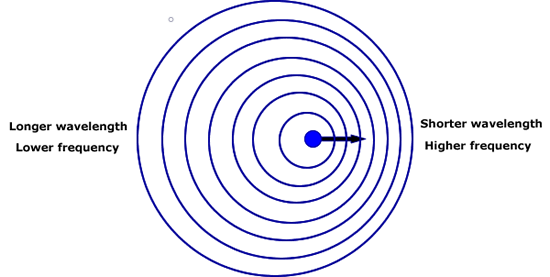
\includegraphics[scale=0.4]{Doppler}
\end{center}

The wavespeed is \(v\) and the source is moving at speed \(v_s\). In this equation \(n'\) means \(n\) after the doppler shift is taken into account. At \(t=0\) the first peak of the wave is emitted. At time \(t=T\) the second peak is emitted. In the time between peaks the first peak has moved distance \(x_1=vT\) and the source has moved distance \(x_2=v_sT\). The distance between the two peaks is:
\[\lambda'=x_1-x_2=vT-v_sT=T(v-v_s)\]
The original wavelength \(\lambda\):
\[\lambda=vT\implies T=\frac{\lambda}{v}\implies\lambda'=\lambda\frac{v-v_s}{v}\]
Finally substituting for \(f\):
\[v=f\lambda\implies\lambda=\frac vf\implies f'=f\frac{v}{v-v_s}\]
As \(v_s\to v\) we get a sonic boom. If both the source and detector are moving and the detector speed is \(v_d\) then the same logic can lead to the equation:
\[f'=f\left(\frac{v\pm v_d}{v\pm v_s}\right)\]
The \(\pm\) is just dependant on the relative directions of the speeds, just think about whether the frequency should increase (source and detector coming together) or decrease (source and detector seperating).
 
\section{}

Linearity is a property of some systems. If \(x\) and \(y\) are solutions to the system then \(x+y\) is also a solution to the system. Differentiation is a linear operator, that is:
\[\diff[2] x(f(x)+g(x)=f'(x)+g'(x)\]

The wave equation is also linear so if \(y_1(x,t)\) and \(y_2(x,t)\) are solutions to the wave equation so is \(y_1+y_2\)

If \(n\) waves are present then the resulting wave is given by:
\[y(x,t)=y_1(x,t)+y_2(x,t)+\cdots y_n(x,t)=\sum_{i=1}^ny_i(x,t)\]

You must take into account the phase difference when you do this calculation.

\subsection*{Example 5.1}

Two waves that are the same but out of phase:
\[y_1(x,t)=A\sin(kx-\omega t),\quad\&\quad y_2=A\sin(kx-\omega t+\varphi)\]
\begin{align*}
y&=y_1+y_2\\
&=A\sin(kx-\omega t)+A\sin(kx-\omega t+\varphi)\\
&=A(\sin(kx-\omega t)+\sin(kx-\omega t+\varphi)\\
\intertext{There is a useful trig identity for this: \(\sin\alpha+\sin\beta=2\sin\left(\frac{\alpha+\beta}{2}\right)\cos\left(\frac{\alpha-\beta}{2}\right)\)}
y&=2A\sin\left(\frac{kx-\omega t+kx-\omega t+\varphi}{2}\right)\cos\left(\frac{kx-\omega t-kx+\omega t-\varphi}{2}\right)\\
&=2A\sin\left(kx-\omega t+\frac{\varphi}{2}\right)\cos\left(\frac{\varphi}{2}\right)\\
&=2A\cos\left(\frac{\varphi}{2}\right)\sin\left(kx-\omega t+\frac{\varphi}{2}\right)
\end{align*}
The new wave that is formed now has amplitude \(2A\cos\left(\frac{\varphi}{2}\right)\) and is \(\frac{\varphi}{2}\) \si{rad} out of phase.

\subsection*{Example 5.2}

Two waves that are the same but traveling in opposite direction:
\[y_1(x,t)=A\sin(kx-\omega t),\quad\&\quad y_2=A\sin(kx+\omega t)\]
\begin{align*}
y&=y_1+y_2\\
&=A\sin(kx-\omega t)+A\sin(kx+\omega t)\\
&=A(\sin(kx-\omega t)+\sin(kx+\omega t)\\
&=2A\sin\left(\frac{kx-\omega t+kx_\omega t}{2}\right)\cos\left(\frac{kx-\omega t-kx+\omega t}{2}\right)\\
&=2A\sin(kx)\cos(\omega t)
\end{align*}
\(\sin(kx)\) is spatial oscillation. \(cos(\omega t)\) is time oscillation.

This is what happens to produce standing waves. A standing wave doesn't move, that means that no energy is transfered. A node is anywhere where \(y(x,t)=0\A x,t\), nodes don't move.

To solve a differential equation you must know the boundary conditions eg. position or speed of the wave at a given time or what is causing the wave. 

\subsection*{Example 5.3}

A standing wave is set up in a string length \(L\) fixed at both ends. What are the boundary conditions of the system?

Since the ends of the string are at positions \(x=0,L\) and they are fixed \((y=0)\) we know that \(y(0,t)=y(L,t)=0\A t\).

We know that \(y(x,t)=2A\sin(kx)\cos(\omega t)\). We need \(\sin(kx)=0\) for \(x=0,L\implies kx=n\pi\, n\in\bb Z,\,n\ne0\implies KL=n\pi\). Substituting in \(k=\frac{2\pi}{\lambda}\) gives \(\lambda=\frac{2L}{n}\)

The longest wavelength \((n=1)\) is the ``fundamental". All shorter wavelengths are ``harmonics". Physical systems usually give a mix of harmonics. Any pattern on the string can be made from a combination of sine nodes.

\subsection*{Example 5.4}

Two waves with different frequencies:

When this occurs the beats phenomonem can be observed, this is the reason that two slightly out of tune notes have a slightly oscillating pitch.

\[y_1(x,t)=A\sin(kx-\omega_1 t),\quad\&\quad y_2=A\sin(kx+\omega \_2t)\]
\begin{align*}
y&=y_1+y_2\\
&=A\sin\left(kx-\omega_1 t\right)+A\sin\left(kx+\omega \_2t\right)\\
&=A(\sin\left(kx-\omega_1t\right)+\sin\left(kx-\omega_2t\right))\\
&=2A\sin\left(\frac{kx-\omega_1t+kx-\omega_2t}{2}\right)\cos\left(\frac{kx-\omega_1t-kx+\omega_2t}{2}\right)\\
&=2A\sin\left(kx-\frac{\omega_1+\omega_2}{2}\right)\cos\left(\frac{\omega_2-\omega_1}{2}t\right)\\
&=2A\sin\left(kx-\bar{\omega}\right)\cos\left(\frac{\Delta \omega}{2}t\right)
\end{align*} 
Where the mean angualr frequency \(\bar\omega=\frac{\omega_1+\omega_2}{2}\) and the difference in angular frequencies \(\Delta\omega=\omega_2-\omega_1\)

\section{}

James Clerk Maxwell showed that light was a wave that followed the following vector calculus:
\[\nabla\cdot\vv E=\frac{\rho}{\varepsilon_0}\]
\[\nabla\cdot\vv B=0\]
\[\nabla\times\vv E=-\vv B\]
\[\nabla\times\vv B=\mu_0(\vv J+\varepsilon_0)\]

From this we can derive wave equations for \(\vv E\) and \(\vv B\). In 1D the equations are:
\[\pd[2]{E}{t}=\frac{1}{\mu_0\varepsilon_0}\pd[2]{E}{x}\]
\[\pd[2]{B}{t}=\frac{1}{\mu_0\varepsilon_0}\pd[2]{B}{x}\]
From this equation we get:
\[v=c=\frac{1}{\sqrt{\mu_0\varepsilon_0}}=\SI{299792458}{m.s^{-1}}\]
A light wave is made of perpendicular waves in the electromagnetic field. The light can be polarised and it can rotate along its axis of travel but the waves always remain perpendicular.

Thomas Young's double slit experiment showed light interfering with itself which is wave behaviour.

Light is not a wave or a particle. It is a quantum object with properties of a wave and a particle. There is no intuitive picture analagous to something that we can see.

We can't see the oscillations of light with time as our eyes don't react fast enough. What we see is the time average of the square of the wave amplitude. That is the time average of the energy of the wave \((E\propto A^2)\).

\subsection*{Light intensity of a sinusoidal wave}

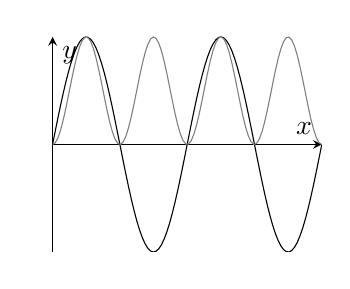
\begin{tikzpicture}
\begin{axis}[
    axis lines = left,
    axis lines = center,
    xtick style={draw=none},
    ytick style={draw=none},
    xticklabels={},
    yticklabels={},
    xlabel = $x$,
    ylabel = {$y$},
]

\addplot [
    domain=0:12.566, 
    samples=100, 
    color=black,
]
{sin(deg(x))};


\addplot [
    domain=0:12.566, 
    samples=100, 
    color=gray,
    ]
    {(sin(deg(x)))^2};

 
\end{axis}
\end{tikzpicture}

This graph shows \(y=\sin x\) and \(y=\sin^2x\).

The intensity \(I\) is given by \(I=\langle|y|^2\rangle_t\) there \(\langle p\rangle_q\) is the average of \(p\) as \(q\) varies.
\[I=\frac 1t\int_0^Ty^2\,dt\]
Here the integral is like taking the mean of a continuous function rather than the discrete data you would usually take the mean of.
\[y=A\sin(\omega t)\]
\[y^2=A^2\sin^2(\omega t)\]
\[I=\frac 1T\in_0^TA^2\sin^2(\omega t)\,dt\]
\[I=\frac{A^2}{T}\left[\frac t2-\frac 14\sin(2\omega t)\right]_0^T\]
At \(t=nT\) for \(n\in\bb Z\) \(\sin(2\omega nT)=\sin(2m\pi)=0\) for \(m\in\bb Z\)
\[I=\frac{A^2}{2}\]
\[I\propto A^2\]

A prisim can split white light showing that it is composed of all other frequencies of visible (and some non-visible) light.

Real instruments (including our eyes) are sensitive to specific wavelength ranges
\[R=\int s(\lambda)I(\lambda)\,d\lambda\]
Where \(R\) is the recieved signal, \(s(\lambda)\) is the sensitivity function and \(I(\lambda)\) is the incoming intensity.

\subsection*{Dispersion}

A pulse of light is made of lots of frequencies of wave together. In free space (a vacuum) all of these travel at the same speed. In any other medium they all travel at different speeds.

The peaks of each frequency travel at a different speed to the whole pacet. We call the speed of the individual frequencies the phase velocity, \(v_p\) and the speed of the whole pacet the qroup velocity, \(v_g\).

In free space light travels at \(c\). In a mediu with refractive index \(n\) light travels at \(\frac cn\) \((n>1)\). In this case \(\omega=ck\) isn't always true. Media have a dispersion relation \(\omega(k)\):
\[v_p=\frac{\omega}{k}\quad\&\quad v_g=\pd{\omega}{k}=\pd{\omega(k)}{k}\]
Often but not always for light \(v_pv_g=c^2\) and \(v_p\ge c,v_g\le c\). It is ok for \(v_p>c\) as no information is being transferred.

In a plasma (ionised gas) free electrons interact with the electromagnetic field giving:
\[\omega=\frac{ck}{\sqrt{1-\frac{\omega_0^2}{\omega^2}}}\]
\[v_p=\frac{\omega}{k}=\frac{c}{\sqrt{1-\frac{\omega_0^2}{\omega^2}}}\]
Note that, for some values of \(\omega\), \(v_p\not\in\bb R\) This is what happens in opaque objects.

\section{}

\[v_g=\pd{\omega}{k}\]
\[\omega=\frac{ck}{\sqrt{1-\frac{\omega_0^2}{\omega^2}}}\]
\[\omega^2=\frac{c^2k^2}{1-\frac{\omega_0^2}{\omega^2}}\]
\[\omega^2\left(1-\frac{\omega_0^2}{\omega^2}\right)=c^2k^2\]
\[\omega^2-\omega_0^2=c^2k^2\]
\[\omega^2=\omega_0^2+c^2k^2\]
\[\omega=\sqrt{\omega_0^2+c^2k^2}\]
\[v_g=\pdiff{k}\left(\omega_0^2+c^2k^2\right)^{-\frac{1}{2}}\]
\[=\frac{c^2k}{\sqrt{\omega_0^2+c^2k^2}}\]

\subsection*{Geometric optics}

Geometric optics is an approximation of light to linear rays travelling in the same direction as the wave.

When light enters a medium it changes speed so that (group) speed is equal to \(v=\frac cn\) where \(n\) is the refractive index of the material. \(n>1\) for all media. \(n=1\) for a vacuum and \(n\approx1\) for air. When light travels across a boundary it can either reflect or refract. Usually it does a combination of both. It depends on the properties of the medium, the light path and the frequency as to what occurs.

\subsection*{Reflection mechanis}

When a light ray is incident on a surface it causes free electrons accelerate which causes them to emit EM radiation which cancels with some waves and not others resulting in only the reflected wave leaving the medium. If the new medium has a higher refractive index then the reflected wave has a phase shift of \(\SI{\pi}{rad}\). If the new medium has a lower refractive index then there is no phase change.

Specular reflection occurs on smooth surfaces with lots of free electrons (metals). Specular reflections preserve the image. Disperse reflections occur in all other cases, usually because at a small enough scale the surface is not flat.

\subsection*{Law of reflection}

\begin{itemize}
\item The incident ray, reflected ray and surface normal are all in the same plane.
\item The angle of incident is the same as the angle of refelection \(\vartheta_i=\vartheta_r\)
\end{itemize}

\begin{center}
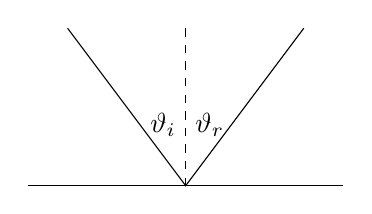
\begin{tikzpicture}[scale=1]
\draw (0,0) -- (4,0);
\draw [dashed] (2,2) -- (2,0);
\draw (0.5,2) -- (2,0) -- (3.5,2);
\node [above left] at (2,0.5) {\(\vartheta_i\)};
\node [above right] at (2,0.5) {\(\vartheta_r\)};
\end{tikzpicture}
\end{center}

\subsection*{Refraction}

\begin{center}
\begin{tikzpicture}
\draw (-4,-2) -- (4,-2) -- (4,2) -- (-4,2) -- (-4,-2);
\draw [ultra thick] (0,2) -- (0,-2);
\draw [dashed] (-4,0) -- (4,0);
\draw (-3,-1) -- (0,0) -- (3,0.5);
\node [below]  at (-2,-2) {\(n_1\)};
\node [below] at (2,-2) {\(n_2\)};
\node [below left] at (-1.2,0) {\(\vartheta_1\)};
\node [above right] at (2,-0.1) {\(\vartheta_2\)};
\end{tikzpicture}
\end{center}

When light passes from an optically less dense to optically more dense material it bends towards the normal and vice versa.

\subsection*{Snell's law}

\[n_1\sin\vartheta_1=n_2\sin\vartheta_2\]

\subsection*{Fermat's principle}

The path taken by light minimise the travel time. (Note that it is a local minimum not a global minimum)

If we define path length \(l=nd\) where \(d\) is the distance travelled and \(n\) is the refractive index then if we have several materials we get:
\[l=\sum_id_in_i\]
and for a continuously changing material:
\[l=\int_{\text{path}}n\,ds\]
where \(ds\) is an element of the path.

The speed of light is given by \(v=\frac cn\) so the time taken to travel \(t\) is given by:
\[t=\frac dv=\frac{d}{\frac{c}{n}}=\frac{nd}{c}=\frac lc\]
From this we can see that \(t\propto l\) so Fermat's principle can be restated as light takes the shortest local path.

Note that for both definitions the paths are local minima and make physical sense.

\subsection*{Derivation of the law of reflection}

\begin{center}
\begin{tikzpicture}[scale=0.75]
\draw (0,-4) -- (0,4);
\draw (6,4) -- (0,0) -- (6,-4);
\draw [dashed] (-2,-4) -- (8,-4);
\draw [dashed] (-2,4) -- (8,4);
\draw [dashed] (-2,0) -- (8,0);
\draw [<->] (8,-4) -- (8,4);
\node [right] at (8,0) {\(y\)};
\draw [<->] (7,0) -- (7,4);
\node [right] at (7,2) {\(y_1\)};
\draw [<->] (7,0) -- (7,-4);
\node [right] at (7,-2) {\(y_2\)};
\node [above left] at (3,2) {\(d_1\)};
\node [below left] at (3,-2) {\(d_2\)};
\node [above] at (1,0) {\(\vartheta_1\)};
\node [below] at (1,0) {\(\vartheta_2\)};
\node [above right] at (6,4) {\(A\)};
\node [below right] at (6,-4) {\(B\)};
\draw [<->] (0,-4.6) -- (6,-4.6);
\draw [dashed] (0,-4) -- (0,-4.6);
\draw [dashed] (6,-4) -- (6,-4.6);
\end{tikzpicture}
\end{center}

There are two local minima in this. One has path length \(y\) and is going from \(A\) straight to \(B\) the other is to reflect off of the surface. To calculate the two angles \(\vartheta_1\) and \(\vartheta_2\) we must find the minimum distance for the light to travel:

Total distance \(D=d_1+d_2\)
By pythagoras we get:
\[d_1^2=y_1^2+x^2\quad\&\quad d_2^2=y_2^2+x^2\]
At the local minimum \(\dv{D}{y_1}=0\):
\[\dv{D}{y_1}=\frac 12\cdot2y_1(y_1^2+x^2)^{\frac 12}+\frac 12\cdot2y_2(y_2^2+x^2)^{\frac 12}\cdot\dv{y_2}{y_1}\]
\[y=y_1+y_2\implies y_2=y-y_1\]
\[\dv{y_2}{y_1}=-1\]
\[\dv{D}{y_1}=\frac{y_1}{\sqrt{y_1^2+x^2}}-\frac{y-y_1}{\sqrt(y-y_1)^2+x^2}=0\]
This is true when \(y_1=y-y_1\implies y_1=\frac 12 y\implies y_1=y_2\)
Since the lengths are equal and all angles are less than \(2\pi\) the angles \(\vartheta_1\) and \(\vartheta_2\) must be the same.

\subsection*{Derivation of Snell's law}

\begin{center}
\begin{tikzpicture}[scale=0.75]
\draw[->] (-1,0) -- (9,0);
\node [right] at (9,0) {\(x\)};
\draw[dashed]  (4,-4) -- (4,4);
\draw (0,4) -- (4,0) -- (5,-4);
\node [above] at (0,4) {\((0,y_1)\)};
\node [below] at (0,0) {\((0,0)\)};
\node [above right] at (4,0) {\((x,0)\)};
\node [above] at (8.5,0) {\(n_1\)};
\node [below] at (8.5,0) {\(n_2\)};
\node [above left] at (4.1,0.3) {\(\vartheta_1\)};
\node [below right] at (3.9,-1.8) {\(\vartheta_2\)};
\node [below] at (5,-4) {\((x_2,y_2)\)};
\node [above right] at (2,2) {\(d_1\)};
\node [right] at (4.5,-2) {\(d_2\)};
\end{tikzpicture}
\end{center}

First by the definition of \(\sin\) we get:
\[\sin\vartheta_1=\frac{x}{\sqrt{x^2+y_1^2}}\quad\&\quad\sin\vartheta_2=\frac{x_2-x}{\sqrt{(x-x_2)^2+y_2^2}}\]
\[l=n_1d_1+n_2d_2\]
\[=n_1\sqrt{(x^2+y_1^2)}+n_2\sqrt{(x-x_2)^2+y_2^2}\]
\[\dv lx=0=\frac{2xn_1}{\sqrt{x^2+y_1^2}}+\frac{2(x-x_2)n_2}{\sqrt{(x-x_2)^2+y_2^2}}\]
\[0=n_1\sin\vartheta_1-n_2\sin\vartheta_2\]
\[n_1\sin\vartheta_1=n_2\sin\vartheta_2\]

Fermat's principle can be derived from Huygen's principle that each wave front acts as a new source of waves in all directions.

\section{}

The radius of curvature of a curve is an approximation of how curved it is given by fitting a circle to part of the curve and taking the radius of the circle.

Expand the function as a taylor series:
\[y=y_0+a(x-x_0)+b(x-x_0)^2+\mathcal{O}(x^3)\]
The \(x^0\) term gives position, the \(x^1\) term gives orientation and the \(x^2\) term gives the curvature.

\begin{center}
\begin{tikzpicture}[scale=2.6]
\draw [domain=-2:2] plot (\x, {0.5*pow(\x,2)});
\draw (0,1) circle [radius=1];
\draw (0,1) -- (0,0);
\node [left] at (0, 0.5) {\(R\)};
\draw (0,1) -- (0.5,0.1339745962);
\node [below right] at (0,0.8) {\(\vartheta\)};
\draw [dashed, <->] (0,0) -- (0.5,0);
\node [below] at (0.25,0) {\(x\)};
\draw [dashed, <->] (0.5,0) -- (0.5,0.1339745962);
\node [right] at (0.5,0.066987) {\(y\)};
\end{tikzpicture}
\end{center}

\[\sin\vartheta\approx\vartheta\quad\&\quad\cos\vartheta\approx1-\vartheta^2\]
\[x=R\sin\vartheta\approx R\vartheta\quad\&\quad y=R(1-\cos\vartheta)\approx R(1-(1-\vartheta^2))=R\vartheta^2\]
\[x^2\approx R^2\vartheta^2\implies\vartheta^2\approx\frac{x^2}{R^2}\implies y=\frac{x^2}{R}\]
Equating coefficients of \(x^2\) with the taylor expansion:
\[bx^2\approx\frac 1Rx^2\implies b\approx\frac 1R\implies R\approx\frac 1b\]

The same can be done in 3D with a sphere to get the radius of curvature of a surface. The radius of curvature has a sign which defines which side of the line the circle is on.

\subsection*{Ray diagrams}

It is convention to have the rays go from left to right and call this direction the positive \(z\) direction, the \(z\) axis is then the same as the optical axis. A lens has two boundaries that a ray must cross with two radii of curvature. The first surface the ray meets is \(R_1\) and the second surface is \(R_2\). By convention a surface that looks like ``(" has positive radius of curvature and a surface that looks like ``)" has negative radius of curvature.

\subsection*{Focal length}

\begin{itemize}
\item Converging lenses have focal length \(f\) which is the displacement from the center of the lens to the plane upon which rays that started parallel will come together. \(f>0\)
\item Diverging lenses have focal length \(f\) which is the displacement from the center of the lens to the plane from where it looks like rays that started parallel emerged when looked at through the lens. \(f<0\)
\end{itemize}

The stronger a lens is the smaller \(|f|\) is. We define power of a lens as \(p=\frac 1f\)

The lens maker's formula:
\[\frac 1f=(n-1)\left(\frac{1}{R_1}-\frac{1}{R_2}\right)\]

A real image is one that can be projected onto a screen and sensed by a detector, it occurs where the rays converge. A virtual image can't be projected on a screen but is where it looks like the light comes from if you view it after it went through the lens.

\begin{center}
\begin{tikzpicture}
\draw (0,0) ellipse (0.2 and 2);
\draw [->] (-3,0) -- (3,0);
\node [right] at (3,0) {\(z\)};
\draw [fill=black] (-2,0) circle (0.1);
\draw [fill=black] (2,0) circle (0.1);
\draw [fill=black] (1,0) circle (0.1);
\node [below] at (-2,-0.1) {Object};
\node [below] at (2,-0.1) {Image};
\node [below] at (1,-0.1) {\(f\)};
\draw [dotted] (0,-2.5) -- (0,2.5);
\draw [dotted] (-2,-2.5) -- (-2,2.5);
\draw [dotted] (2,-2.5) -- (2,2.5);
\draw [dotted] (1,-2.5) -- (1,2.5);
\draw [|-|] (-2,2.5) -- (0,2.5);
\draw [|-|] (0,2.5) -- (2,2.5);
\draw [|-|] (0,-2.5) -- (1,-2.5);
\node [above] at (-1,2.5) {\(u\)};
\node [above] at (1,2.5) {\(v\)};
\node [below] at (0.5,-2.5) {\(f\)};
\end{tikzpicture}
\end{center}

By convention when they are the side of the lens that they are in the diagram \(f,u,v>0\)

Rules for thin lens, paraxial (small angle) approximation:
\begin{itemize}
\item Rays through the centre of the lens don't change direction
\item Rays that come in parallel end on the focal plane
\item Rays from the focal plane end up in parallel
\end{itemize}

\begin{center}
\begin{tikzpicture}[scale=2]
\draw (0,0) ellipse (0.2 and 2);
\draw [->] (-3,0) -- (3,0);
\node [right] at (3,0) {\(z\)};
\draw [->, ultra thick] (-2,0) -- (-2,1);
\draw [->, ultra thick] (2,0) -- (2,-1);
\draw [fill=black] (1,0) circle (0.025);
\node [below] at (1,0) {\(f\)};
\draw [dotted] (0,-2.5) -- (0,2.5);
\draw [dotted] (-2,-2.5) -- (-2,2.5);
\draw [dotted] (2,-2.5) -- (2,2.5);
\draw [dotted] (1,-2.5) -- (1,2.5);
\draw [|-|] (-2,2.5) -- (0,2.5);
\draw [|-|] (0,2.5) -- (2,2.5);
\draw [|-|] (0,-2.5) -- (1,-2.5);
\node [above] at (-1,2.5) {\(u\)};
\node [above] at (1,2.5) {\(v\)};
\node [below] at (0.5,-2.5) {\(f\)};
\draw [gray] (-2,1) -- (3,-1.5);
\draw [gray] (-2,1) -- (0,1) -- (3,-2);
\node [left] at (-2,0.5) {\(h_0\)};
\node [right] at (2,-0.5) {\(h_1\)};
\node [above left] at (-0.35,-0.05) {\(A\)};
\node [below right] at (0.35,0) {\(A\)};
\node [above left] at (0.9,-0.05) {\(B\)};
\node [below right] at (1.1,0.01) {\(B\)};
\end{tikzpicture}
\end{center}

By convention an inverted image has negative height
\[\frac{h_0}{u}=\tan A=\frac{-h_1}{v}\]
Magnification is the ratio of the image height to the object height:
\[M=\frac{h_1}{h_2}=-\frac vu\]
\[\frac{h_0}{f}=\tan B=\frac{-h_1}{v-f}\]
\[\implies-\frac{h_1}{h_0}=\frac{v-f}{f}\]
\[\implies\frac vu=\frac{v-f}{f}\]
\[=\frac vf-\frac ff\]
\[=\frac vf-1\]
\[\implies\frac vu=\frac vf-1\]
\[\implies\frac 1u=\frac 1f-\frac 1v\]
\[\implies\frac 1f=\frac 1u+\frac 1v\]

This is known as the Gaussian lens equation.

If \(v>0\) then the image is real. If \(v<0\) then the image is virtual. For \(v>0\) we need \(f>0\) and \(u>f\). Since when this occurs \(u,v>0\) \(M=-\frac vu<0\) so the image is inverted. For \(v<0\) either \(f>0\) and \(u<f\), so \(M>1\), so the image is upright and magnified, or \(f<0\) so \(M>0\) so the image is upright.

\section{}

\subsection*{Multiple lenses}

The image of the first lens becomes the object for the second lens. This rule still applies for virtual images, negative lenses and images on the opposite side of the lens.

From the last lecture we have \(M=-\frac vu\). The height  of the 1\(^{\text{st}}\) image is \(h_1=M_1h_0\). The height of the 2\(^{\text{nd}}\) image is \(h_2=M_2h_1\). The total magnification is:
\[M_{tot}=\frac{h_2}{h_0}=\frac{M_2h_1}{\frac{h_1}{M_1}}=M_1M_2\]
This is true for all \(M\) including \(M<0\) and \(|M|<1\).

\subsection*{Lenses in contact}
\begin{center}
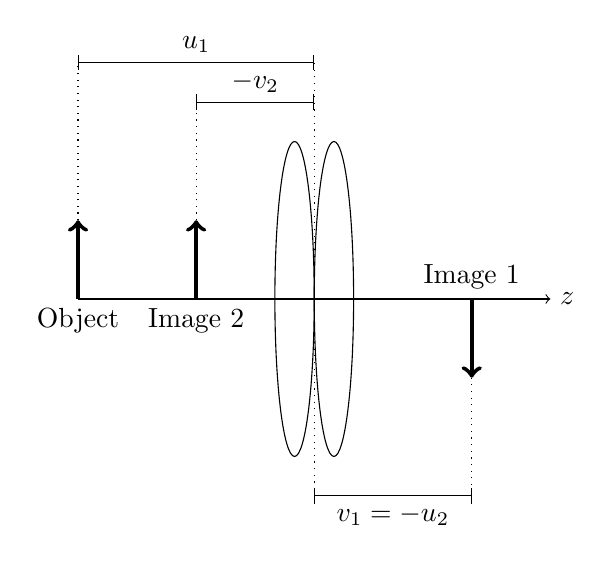
\begin{tikzpicture}
\draw [->] (-3,0) -- (3,0);
\node [right] at (3,0) {\(z\)};
\draw (-0.25,0) ellipse (0.25 and 2);
\draw (0.25,0) ellipse (0.25 and 2);
\draw [->, ultra thick] (-3,0) -- (-3,1);
\draw [->, ultra thick] (-1.5,0) -- (-1.5,1);
\draw [->, ultra thick] (2,0) -- (2,-1);
\node [below] at (-3,0) {Object};
\node [below] at (-1.5,0) {Image 2};
\node [above] at (2,0) {Image 1};
\draw [dotted] (-3,1) -- (-3,3);
\draw [dotted] (-1.5,1) -- (-1.5,2.5);
\draw [dotted] (2,-1) -- (2,-2.5);
\draw [dotted] (0,-2.5) -- (0,3);
\draw [|-|] (-3,3) -- (0,3);
\draw [|-|] (-1.5,2.5) -- (0,2.5);
\node [above] at (-0.75,2.5) {\(-v_2\)};
\node [above] at (-1.5,3) {\(u_1\)};
\draw [|-|] (0,-2.5) -- (2,-2.5);
\node [below] at (1,-2.5) {\(v_1=-u_2\)};
\end{tikzpicture}
\end{center}
The gaussian lens equation:
\[\frac 1u+\frac 1v=\frac 1f\]
Applying the gaussian lens equation for lens 1:
\[\frac{1}{u_1}+\frac{1}{v_1}=\frac{1}{f_1}\]
\[\implies \frac{1}{v_1}=\frac{1}{f_1}-\frac{1}{u_1}\tag{9.1}\]
Applying the gaussian lens equation for lens 2:
\[\frac{1}{u_2}+\frac{1}{v_2}=\frac{1}{f_2}\]
\[\implies \frac{1}{v_2}=\frac{1}{f_2}-\frac{1}{u_2}\]
\[v_1=-u_2\implies\frac{1}{v_2}=\frac{1}{f_2}+\frac{1}{v_1}\]
Substituting in (9.1) gives:
\[\frac{1}{v_2}=\frac{1}{f_2}+\frac{1}{f_1}-\frac{1}{u_1}\]
\[\frac{1}{v_2}+\frac{1}{u_1}=\frac{1}{f_2}+\frac{1}{f_1}\]
Let \(F\) be the effective focus distance of the system:
\[\frac 1F=\frac{1}{v}+\frac{1}{u}\]
\[\implies \frac{1}{F}=\frac{1}{f_1}+\frac{1}{f_2}=\frac{1}{v_2}+\frac{1}{u_1}\]
So the whole system is the same as a single lens with effective focal length \(F\), object distance \(u_1\) and image distance \(v_2\). This shows that focal lengths add in parralel for lenses in contact. This can also be written as powers adding in series as \(P=p_1+p_2\)

\subsection*{Compound microscopes}

Compound microscopes are made from two converging lenses. Image 1 is real and between the two lenses. Image 2 is virtual and further away than the object. You can see the virtual image as you eye is another lens that makes the image real again. The total magnification is given by \(M=M_1M_2\).

\begin{center}
\begin{tikzpicture}
\draw [->] (-5,0) -- (5,0);
\node [right] at (5,0) {\(z\)};
\draw (-2,0) ellipse (0.25 and 2);
\draw (2,0) ellipse (0.25 and 2);
\draw [->, ultra thick] (-5,0) -- (-5,1);
\node [below] at (-5,0) {Object};
\draw [|-|] (-5,2.5) -- (-2,2.5);
\draw [|-|] (-2,2.5) -- (0,2.5);
\draw [|-|] (0,2.5) -- (2,2.5);
\draw [|-|] (2,2.5) -- (5,2.5);
\node [above] at (-3.5,2.5) {\(u_1\)};
\node [above] at (-1,2.5) {\(v_1\)};
\node [above] at (1,2.5) {\(u_2\)};
\node [above] at (3.5,2.5) {\(v_2\)};
\draw [|-|] (-2,-2.5) -- (2,-2.5);
\node [below] at (0,-2.5) {\(d\)};
\end{tikzpicture}
\end{center} 

Applying the gaussian lens equation to both lenses:
\[\frac{1}{v_1}=\frac{1}{f_1}-\frac{1}{u_1}\qquad\frac{1}{v_2}=\frac{1}{f_2}-\frac{1}{u_2}=\frac{1}{f_2}-\frac{1}{d-v_1}\]
We want the rays from the second image to be parallel as this makes the eye relax so the microscope is easier to use. This means that \(v_2\to\infty\):
\[\lim_{v_2\to\infty}\frac{1}{u_2}+\frac{1}{v_2}=\frac{1}{u_2}=\frac{1}{f_2}\implies u_2=f_2\tag{9.2}\]
It can be seen from the diagram that:
\[u_2+v_1=d\implies v_1=d-u_2\]
If we subsititute (9.2) into this we get:
\[v_1=d-f_2\tag{9.3}\]
If we substitute (9.3) into the gaussian lens equation for lens 1 we get:
\[\frac{1}{u_1}=\frac{f_1}-\frac{d-f_2}=\frac{1}{f_1}+\frac{1}{f_2-d}\]
Since we want the waves to end up parallel then we want the object at the focal distance from the lens so \(u_1=F\) so we get that:
\[\frac 1F= \frac{1}{f_1}+\frac{1}{f_2-d}\]

If \(d=0\) then we get the equation for lenses in contact.

\subsection*{Telescopes}

When and object is viewed through a telescope the object is far enough away that we can assume the light rays are parallel. This means that \(u_1\to\infty\). We also want the rays to come out parallel so \(v_2\to\infty\)

The simplest telescope is the gallilean telescope. It is made of a converging and a diverging lens which are set up such that they have there focal point in the same spot. The distance between the lenses is \(d\).
The gaussian lens equation for the first lens as \(u_1\to\infty\):
\[\lim_{u_1\to\infty}\frac{1}{u_1}+\frac{1}{v_1}=\frac{1}{v_1}=\frac{f_1}\implies v_1=f_1\]
The gaussian lens equation for the second lens as \(v_2\to\infty\):
\[\lim_{v_2\to\infty}\frac{1}{u_2}+\frac{1}{v_2}=\frac{1}{u_2}=\frac{f_2}\implies u_2=f_2\]
The magnification is given by:
\[M=-\frac{v_2}{u_1}=\lim_{u_1,v_2\to\infty}=-\frac{\infty}{\infty}\]
This is not a valid answer \Sadey[1.25]


\section{}
If instead we consider the angle \(\vartheta_o\) between the optical axis and the incoming ray which goes through the center of the objective lens. This angle is also made by the ray and the optical axis on the other side of the lens. This forms a right angle triangle between the center of the lens, and the top and bottom of the image. If the image height is \(h\) and the focal length is \(f_o\) then we get the relationship:
\[\tan\vartheta_o=\frac{h}{f_o}\approx\vartheta_o\tag{10.1}\]

If we now consider the angle \(\vartheta_e\) between the optical axis and the ray passing through the center of the eyepiece lens. This angle is part of the right angle triangle fomed between the center of the eyepiece lens, and the top and bottom of the object of the eyepiece lens (which is the image of the objective lens). We get the relationship:
\[\tan\vartheta_e=\frac{h}{f_e}\approx\vartheta_e\tag{10.2}\]

Combining (10.1) and (10.2) we get:
\[\frac{\vartheta_o}{\vartheta_e}\approx\frac{f_e}{f_o}\]

\subsection*{Diffraction}

Diffraction and inteference are a set of phenomona that occur when waves encounter objects about the size of their wavelenght.

In 1D with waves with phase \(\varphi\):
\[y_1+y_2=2A\cos\left(\frac{\varphi}{2}\right)\sin\left(kx-\omega t+\frac{\varphi}{t}\right)\]

\(\cos\left(\frac{\varphi}{2}\right)\) is the phase factor when \(\cos\left(\frac{\varphi}{2}\right)=0\) the waves cancel. In 2D the phase factor is a function of position.

~\makebox[0pt][c]{\rotatebox[origin=c]{90}{( )}} ~These waves are antiphase, they will cancel out, this is called destructive inteference.

~\makebox[0pt][c]{\rotatebox[origin=c]{270}{( (}} ~These waves are in phase, they will add up, this is called constructive inteference.

The difference in path lengths determins how they intefere. For two waves one of which has traveled a distance \(x_1\) and the other \(x_2\) the sum of the two waves is:
\[y_1+y_2=2A\sin\left(k\frac{x_1+x_2}{2}-\omega t\right)\cos\left(k\frac{x_1-x_2}{2}\right)\]

The first term oscilates with time. The second term effects amplitude at different points.
\[I\propto \cos^2\left(k\frac{x_1-x_2}{2}\right)=\cos^2\left(\pi\frac{x_1-x_2}{\lambda}\right)\]

So if the distances differ by an integer number of wavelengths then the waves will be in phase. If it differs by a half integer number of wavelengths then the waves will be out of phase.

\subsection*{Double slit}

\begin{center}
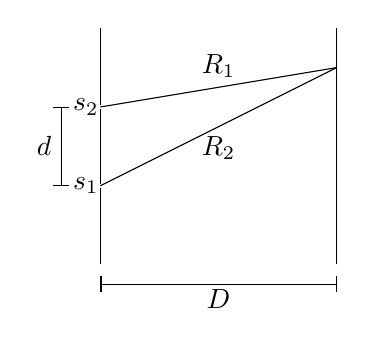
\begin{tikzpicture}[scale=0.5]
\draw (0,0) -- (0,1.95);
\draw (0,2.05) -- (0,3.95);
\draw (0,4.05) -- (0,6);
\node [left] at (0.2,2) {\(s_1\)};
\node [left] at (0.2,4) {\(s_2\)};
\draw [|-|] (-1,2) -- (-1,4);
\node [left] at (-1,3) {\(d\)};
\draw (6,0) -- (6,6);
\draw [|-|] (0,-0.5) -- (6,-0.5);
\node [below] at (3,-0.4) {\(D\)};
\draw (0,2) -- (6,5);
\draw (0,4) -- (6,5);
\node [above] at (3,4.5) {\(R_1\)};
\node [below] at (3,3.5) {\(R_2\)};
\end{tikzpicture}
\end{center}

In general this problem is quite hard to solve but it is simpler when \(D\gg d\) as rays \(R_1\) and \(R_2\) are basically parallel:

\begin{center}
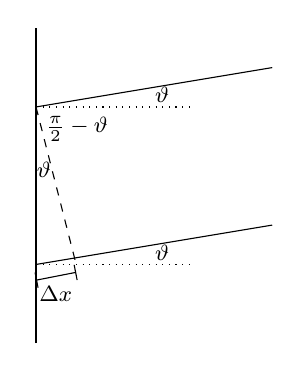
\begin{tikzpicture}
\draw (0,0) -- (0,4);
\draw (0,3) -- (3,3.5);
\draw (0,1) -- (3,1.5);
\draw [dotted] (0,3) -- (2,3);
\draw [dotted] (0,1) -- (2,1);
\draw [dashed] (0,3) -- (0.51,1);
\node at (1.6,3.15) {\footnotesize{\(\vartheta\)}};
\node at (1.6,1.15) {\footnotesize{\(\vartheta\)}};
\node at (0.1,2.2) {\footnotesize{\(\vartheta\)}};
\node [below right] at (0,3) {\footnotesize{\(\frac{\pi}{2}-\vartheta\)}};
\draw [|-|] (0,0.8) -- (0.51,0.9);
\node [below] at (0.25,0.85) {\footnotesize{\(\Delta x\)}};
\end{tikzpicture}
\end{center}

The path difference is \(\Delta x=d\sin\vartheta\). There are maxima at \(\Delta x=m\lambda\) for \(m\in\bb Z\) therefore there are maxima at:
\[m\lambda=d\sin\vartheta\]
Minima are at:
\[\left(m+\frac 12\right)\lambda=d\sin\vartheta\]

\subsection*{Diffraction gratings}

A diffraction grating is a regularly spaced grid of slits, usually engraved on glass.

\begin{center}
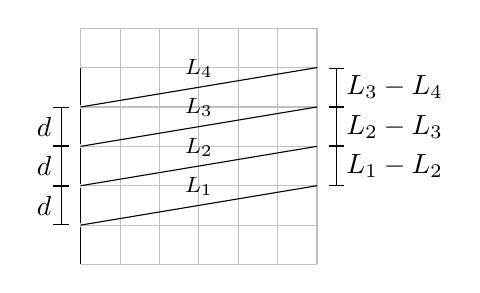
\begin{tikzpicture}[scale=0.5]
\draw [lightgray] (0,0) grid (6,6);
\draw (0,0) -- (0,0.95);
\draw (0,1.05) -- (0,1.95);
\draw (0,2.05) -- (0,2.95);
\draw (0,3.05) -- (0,3.95);
\draw (0,4.05) -- (0,5);
\draw [|-|] (-0.5,1) -- (-0.5,2);
\draw [|-|] (-0.5,2) -- (-0.5,3);
\draw [|-|] (-0.5,3) -- (-0.5,4);
\node [left] at (-0.5,1.5) {\(d\)};
\node [left] at (-0.5,2.5) {\(d\)};
\node [left] at (-0.5,3.5) {\(d\)};
\draw (0,1) -- (6,2);
\draw (0,2) -- (6,3);
\draw (0,3) -- (6,4);
\draw (0,4) -- (6,5);
\draw [|-|] (6.5,2) -- (6.5,3);
\draw [|-|] (6.5,3) -- (6.5,4);
\draw [|-|] (6.5,4) -- (6.5,5);
\node [right] at (6.5,2.5) {\(L_1-L_2\)};
\node [right] at (6.5,3.5) {\(L_2-L_3\)};
\node [right] at (6.5,4.5) {\(L_3-L_4\)};
\node [above] at (3,1.5) {\footnotesize{\(L_1\)}};
\node [above] at (3,2.5) {\footnotesize{\(L_2\)}};
\node [above] at (3,3.5) {\footnotesize{\(L_3\)}};
\node [above] at (3,4.5) {\footnotesize{\(L_4\)}};
\end{tikzpicture}
\end{center}

Making the same assumption as for single slit that \(D\gg d\) so the rays are basically parallel
\[L_1-L_2=L_2-L_3=L_3-L_4=\cdots=d\sin\vartheta\]
\[L_1-L_3=(L_1-L_2)+(L_2-L_3)=d\sin\vartheta+d\sin\vartheta=2d\sin\vartheta\]
In general:
\[L_1-L_{n+1}=nd\sin\vartheta\]
This is generally quite complicated but we know that any two neighbouring rays are in phase as if they where in a double slit experiment. This means that if \(L_1\) and \(L_2\) are in phase then \(L_2\) and \(L_3\) are in phase so by strong induction we know that if \(L_1\) and \(L_2\) are in phase then \(L_1\) is in phase with all other rays. This means that there are maxima at \(m\lambda=d\sin\vartheta\).

The pattern of light depends on \(k\) since \(k=\frac{2\pi}{\lambda}\)
\begin{align*}
m\lambda&=d\sin\vartheta\\
\intertext{For the first fringe:}
\lambda&=d\sin\vartheta\\
\vartheta&\approx\sin\vartheta\\
\lambda&\approx d\vartheta\\
\frac{\lambda}{d}&\approx\vartheta
\end{align*}

This means light will be split into its wavelengths with red light further out than blue. The central fringe will be white.

\section{}
Wavefronts are points/lines/surfaces of constant phase. The exact choice of phase is arbitrary. In 1D it is a series of points traveling with the wave. In 2D it is a line. Wavefronts travel perpendicularly to the energy.

\subsection*{Huygen's principal (HP)}

\begin{displayquote}
Each point of the wavefront acts as a new source of hemispherical ``wavelets" moving in the forward direction
\end{displayquote}

This isn't a fundamental science law but a model. It arrises from a method of solving the underlying wave equation using Green's functions. We can use it to understand diffraction. Each point of the wavefront is creating new wavelets which then create a new wavefront so when a block is discovered the wavefront will create new wavelets which can go around it. The number of wavelets considered isn't important as long as you use enough to get a good picture of what is happening.

It is also possible to derive Snell's law from Huygen's principal:

\begin{center}
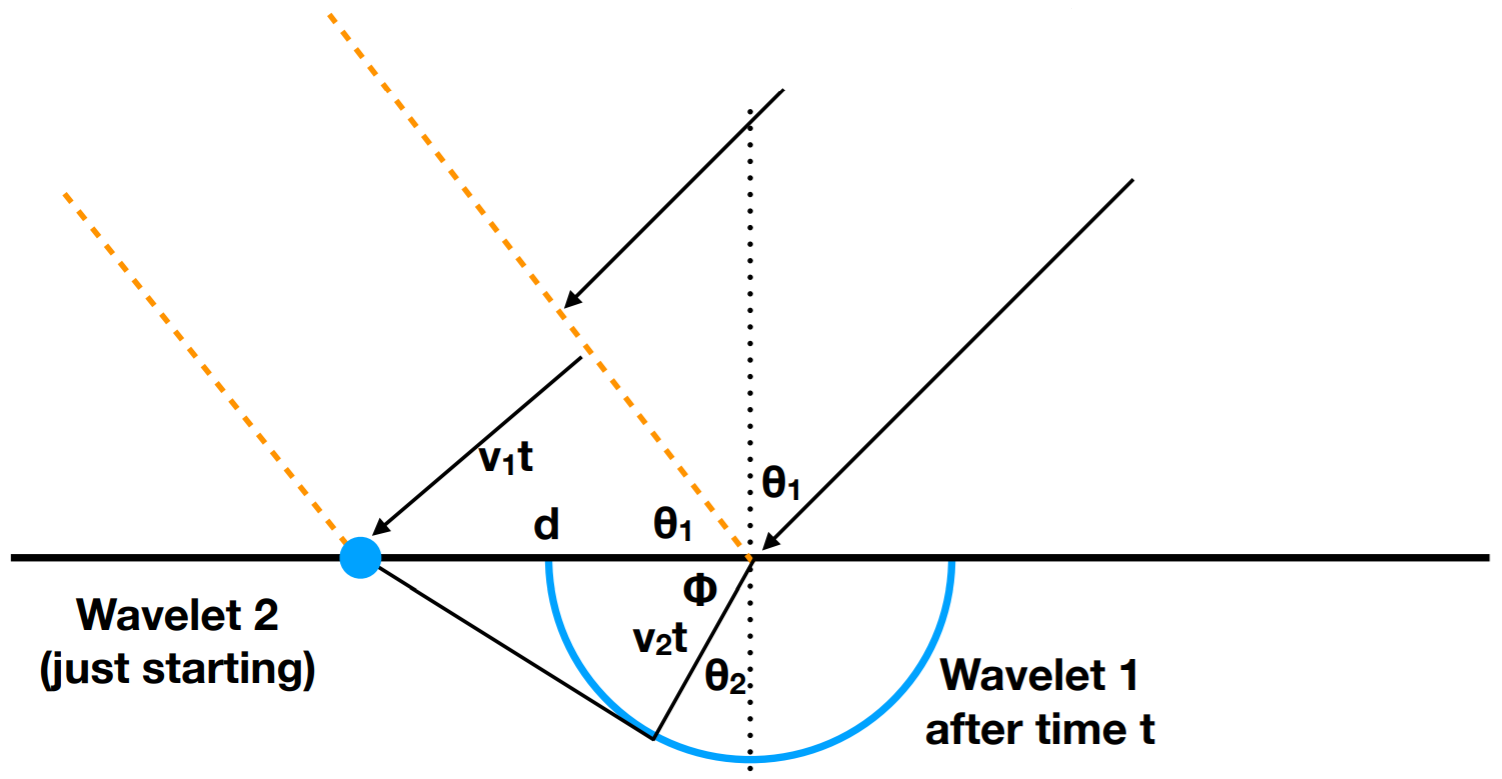
\includegraphics[scale=0.3]{HuygensSnellsLaw}
\end{center}

If the wave starts in a medium with refractive index \(n_1\) and travels with velocity \(v_1\) then moves into a medium with refractive index \(n_2\) where it travels with velocity \(v_2\). At time \(t=0\) the first part of the wavefront enters the second medium and creates a wavelet. and at time \(t\) the second ray enters the new medium. By comparing expressions for \(d\) we get Snell's law:
\[\sin \vartheta_1=\frac{v_1t}{d}\]
\[\varphi = \frac{\pi}{2}-\vartheta_2\]
\[\cos\varphi=\frac{v_2t}{d}=\sin\vartheta_2\]
\begin{align*}
d=\frac{v_1t}{\sin\vartheta_1}&=\frac{v_2t}{\sin\vartheta_2}\\
\frac{\sin\vartheta_1}{v_1}&=\frac{\sin\vartheta_2}{v_2}\\
\frac{c\sin\vartheta_1}{v_1}&=\frac{c\sin\vartheta_2}{v_2}\\
n_1\sin\vartheta_1&=n_2\sin\vartheta_2
\end{align*}

It is also possible to derive the double slit inteference pattern by considering two slits that are thin enough that only one wavelet can get through. Since this is a physicaly impossible system we can consider one slit inteference:

\begin{center}
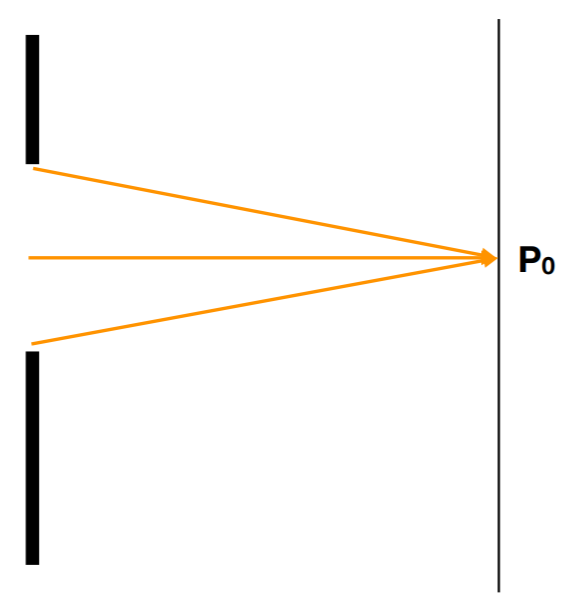
\includegraphics[scale=0.3]{SingleSlit1}
\end{center}

There is a bright fringe at \(P_0\) because if the distance to the screen is much bigger than the slit width then the rays are approximately parallel. Each pair of rays at equal distance apart has the same path difference so it is only necessary to consider one pair:

\begin{center}
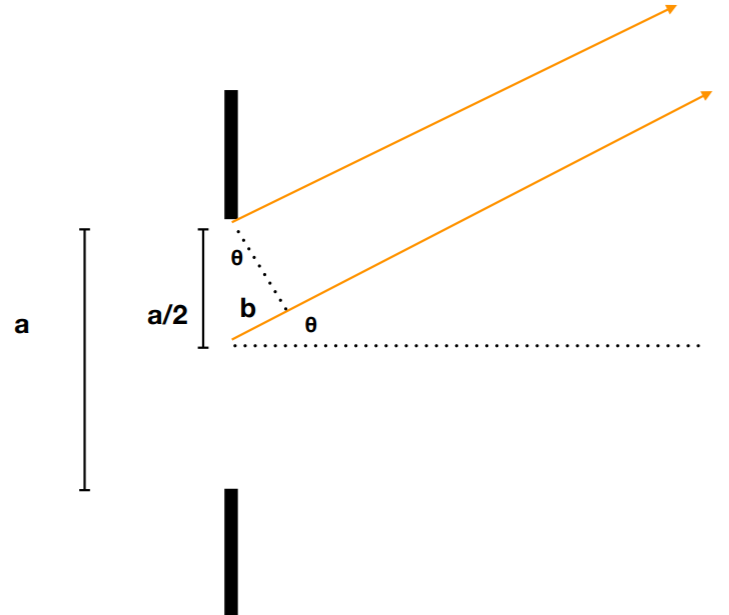
\includegraphics[scale=0.3]{SingleSlit2}
\end{center}

As with the double slit cancelation occurs when \(b=\frac a2\sin\vartheta\). First order cancelation \(\frac{\lambda}{2}=b=\frac a2\sin\vartheta\) So there are minima at \(\lambda=a\sin\vartheta\). So for the complete single slit:
\[b=x\sin\vartheta\]
\begin{align*}
A_x &= A_0\sin(k(D-b)-\omega t)\\
&= A_0\sin(kD-kx\sin\vartheta-\omega t)\\
&= A_0[\sin(kD-\omega t)cos(kx\sin\vartheta)-\cos(kD-\omega t)\sin(kx\sin\vartheta)]
\end{align*}
Where \(x\) is the distance from the center of the slit.

\section{}

A crystal is a solid with a repeating molecular structure. It has planes of molecules:

\begin{center}
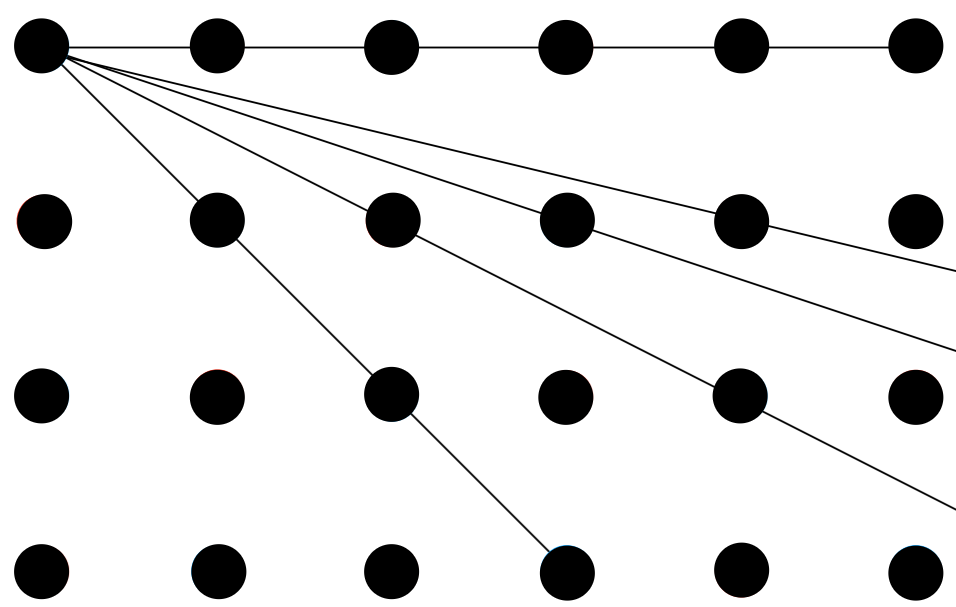
\includegraphics[scale=0.2]{CrystalPlanes}
\end{center}

The distance between planes is approximately \(10^{-10}\) which is about the same as the wavelength of x-rays therefore x-rays will defract in a crystal. The different layers of the crystal act as a diffraction grating.

\subsection*{X-ray crystalography - single crystal}

When an x-ray is incident on a crystal if it hits a molecule a diffuse reflection occurs. Most of the reflected rays will cancel leaving rays at only specific angles with perfecly constructive inteference. If we consider only the rays that don't cancel:

\begin{center}
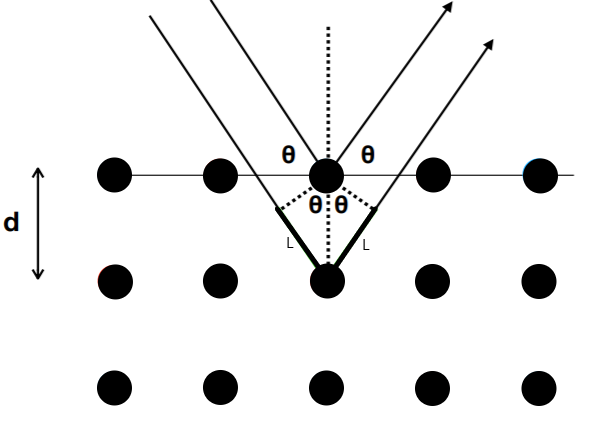
\includegraphics[scale=0.4]{CrystalReflection}
\end{center}

The two rays leaving are close enough to intefere. The path difference \(\Delta\) is given by:
\[\Delta = 2L=2d\sin\vartheta\]
So the inteference is constructive if:
\[m\lambda=2d\sin\vartheta\text{ for }m\in\bb Z\]
Note that \(\vartheta\) is not the angle of incidence \(\vartheta_i\) but rathter \(\vartheta = \frac{\pi}{2}-\vartheta_i\).

This is Bragg's law

Each plane has different spacing so there are different angles of reflection depending on the angle the light is shone.

\subsection*{X-ray crystalography - powdered crystal}

In reality a powederd crystal is used. This results in a circular diffraction pattern.

\begin{center}
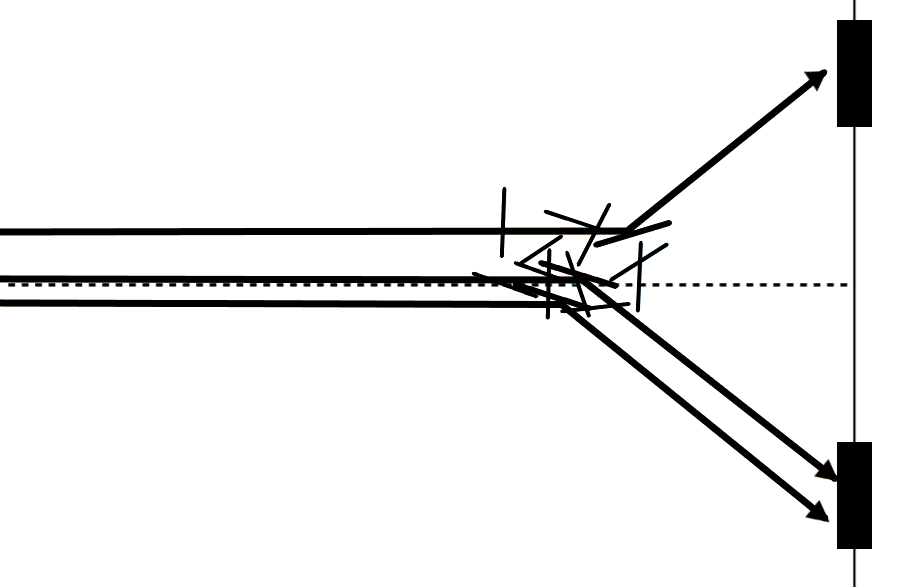
\includegraphics[scale=0.2]{CrystalPowder}
\end{center}

\subsection*{Thin Film Inteference}

A thin film will cause light reflecting off of the two edges of the film to intefere with itself. We imagine light normal to the surface of the film. The path difference length is affected by three factors:
\begin{itemize}
\item Physical length difference
\item Refractive index (\(n_{\text{film}}>n_{\text{air}}\))
\item Phase shift on reflection from surface of higher refractive index by \(\si{\pi rad}\) 
\end{itemize}
This results in a phase difference \(\Delta\varphi\) for a film thickness \(L\)
\[\Delta\varphi=2kL-\pi\]
The first term \(2kL\) is due to the physical length difference. The second term \(\pi\) is due to the reflection. \(k\) is the wavenumber in the film. \(k = k_{\text{film}}=\frac{2\pi}{\lambda_{\text{film}}}\). \(\omega\) is constant and \(v\) changes.
\[\lambda_{\text{film}}=\frac{\lambda_{\text{air}}}{n_{\text{film}}}\]
\[\implies\Delta\varphi=\frac{4\pi nL}{\lambda}-\pi\]
Constructive inteference occurs if \(\Delta\varphi=2m\pi\) hence \(2L = \left(m+\frac 12\right)\frac{\lambda}{n}\) and destructive inteference occurs if \(\Delta\varphi=(2m+1)\pi\) hence \(2L = \frac{m\lambda}{n}\) for \(m\in\bb Z\)

\subsection*{Uses of interference}

\begin{itemize}
\item Interferometer - A genereal class of tools using path difference for measurement
\item Radio interferometry - Multiple radiotelescopes aproximately \SI{10}{km} apart with correlated ouputs that act as a \SI{10}{km} wide telescope. It can only see small stuff as \(\sin\vartheta\propto\frac{\lambda}{d}\)
\item The Michelson-Morley experiment (which shows there is no aether)
\item LIGO (which discovered gravitational waves)
\end{itemize}

\part{Quantum Physics}
\section{}

The photoelectric effect implies that light has particle nature. When a light is shon on a photo emmitter it causes electrons to be emitted following the following equation:
\[eV_s=hf-\varphi\]
Where \(e\) is the charge of an electron, \(V_s\) is the stopping voltage required to stop current flow, \(h\) is plank's constant \(h=\num{6.626e-34}\), \(f\) is the frequency of the incident light and \(\varphi\) is the workfunction which is the value \(hf_0\) such that \(hf-hf_0=0\) where \(f_0\) is the minimum frequency.

When shone on a slit electrons will diffract, this shows that they have wave like nature.

\subsection*{Wave function}

The wave function \(\psi\) is a multivariable function \(\psi(x,y,z,t)\) where \(x,y\) and \(z\) are the three spatial dimensions and \(t\) is time. For this course we will only look at one dimensional functions which are time independant (time doesn't effect the potential energy of the particle). These take the form \(\psi(x)\). An example would be \(\psi_+\):
\[\psi_+(x)=Ae^{ikx}\]
where \(A\) and \(k\) are constants. There is another solution closely linked to this one and also both can be written in a different form:
\[\psi_+(x)=Ae^{ikx}=A(\cos kx+i\sin kx)\qquad\psi_-(x)=Ae^{-ikx}=A(\cos kx-i\sin kx)\]
These are waves. It is possible to work out the probability of the wave being found in a particular space using the probability function \(|\psi|^2=\psi\cc\psi\). For the example \(\psi=Ae^{ikx}\):
\[\psi=Ae^{ikx}\implies\cc\psi=Ae^{-ikx}\]
\[|\psi|^2=\psi\cc\psi=Ae^{ikx}Ae^{-ikx}=A^2e^{ikx-ikx}=A^2\]
This is independant of \(x\) and therefore the particle is equally likely to be at any point in space.

\subsection*{The Schr\"odinger equation}

\begin{center}
\boxed{\dv[2]{\psi}{x}+\frac{8\pi^2m}{h^2}[E-U(x)]\psi=0}
\end{center}

In this equation \(m\) is the mass of the particle, \(E\) is the total energy of the system and \(U(x)\) is the potential energy of the system. For the case where \(U(x)\) is independant of \(x\) since the point at wich \(U(x)=0\) is arbitrary we can just set it equal to 0 so we get:
\[\dv[2]{\psi}{x}+\frac{8\pi^2m}{h^2}E\psi=0\]

It is possible to show that our example from before satisfies the equation under certain conditions:
\begin{align*}
\psi&=Ae^{ikx}\\
\dv{\psi}{x}&=Aike^{ikx}\\
\dv[2]{\psi}{x}&=-Ak^2e^{ikx}
\end{align*}

Substituting into the Schr\"odinger equation:
\[-Ak^2e^{ikx}+\frac{8\pi^2m}{h^2}EAe^{ikx}=0\]
\[-k^2+\frac{8\pi^2m}{h^2}E=0\]
So \(\psi=Ae^{ikx}\) is a solution if:
\[E=\frac{h^2k^2}{8\pi^2m}\iff k^2=\frac{8\pi^2mE}{h^2}\]

The reduced plank's constant \(\bar h\) is defined as \(\bar h\triangleq\frac{h}{2\pi}\). Using this we can write the conditions as:
\[E=\frac{\hb^2k^2}{2m}\iff k^2=\frac{mE}{\hb^2}\]
Note that this only applies for a free particle (a particle with a boudary will have \(U(x)\) that depends on \(x\)). The whole Schr\"odinger equation can be written as:
\[\dv[2]{\psi}{x}+\frac{2m}{\hb^2}[E-U(x)]\psi=0\]


\section{}

Using \(\hb\) we get \(E=\hb\omega\)

From last lecture we saw that if \(\psi_+=Ae^{ikx}\) is a solution then \(k^2=\frac{8\pi^2m}{h^2}E\) If this is true then the Scr\"odinger equation can be rewritten as:
\[\dv[2]{\psi}{x}+k^2\psi=0\]
This is the wave equation.

\(k\) is the wave number in this equation. It is the number of waves per unit distance.

\[k^2=\frac{8\pi^2m}{h^2}E\implies E=\frac{k^2h^2}{8\pi^2m}\]
For non relativistic particles \(E=\frac{p^2}{2m}=\frac{m^2v^2}{2m}=\frac12mv^2\)
\[E=\frac{h^2k^2}{8\pi^2m}=\frac{p^2}{2m}\]
\[p^2=\frac{h^2k^2}{4\pi^2}\]
\[p=\frac{hk}{4\pi^2}=\hb k\]
The momentum \(p\) of a solution to the free Scr\"odinger equation is given by \(p=\hb k\)

A more realistic solution to the Schr\"odinger equation is the sum of sinusoidal terms of different frequencies:
\[\psi(x)=\sum_jAe^{ik_jx}\]

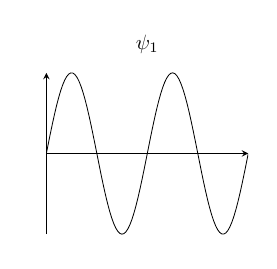
\begin{tikzpicture}[scale=0.75]
\begin{axis}[
    title={\(\psi_1\)},
    axis lines = left,
    axis lines = center,
    xtick style={draw=none},
    ytick style={draw=none},
    xticklabels={},
    yticklabels={},
    xlabel = {},
    ylabel = {},
]

\addplot [
    domain=0:12.566, 
    samples=100, 
    color=black,
]
{sin(deg(x))};
 
\end{axis}
\end{tikzpicture}
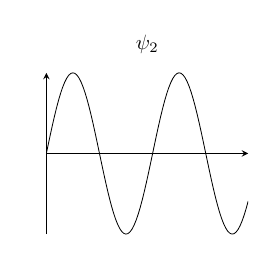
\begin{tikzpicture}[scale=0.75]
\begin{axis}[
    title={\(\psi_2\)},
    axis lines = left,
    axis lines = center,
    xtick style={draw=none},
    ytick style={draw=none},
    xticklabels={},
    yticklabels={},
    xlabel = {},
    ylabel = {},
]

\addplot [
    domain=0:12.566, 
    samples=100, 
    color=black,
]
{sin(deg(0.95*x))};
 
\end{axis}
\end{tikzpicture}
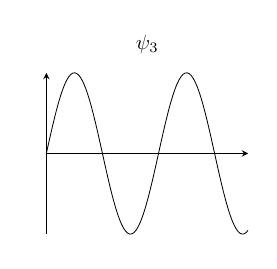
\begin{tikzpicture}[scale=0.75]
\begin{axis}[
    title={\(\psi_3\)},
    axis lines = left,
    axis lines = center,
    xtick style={draw=none},
    ytick style={draw=none},
    xticklabels={},
    yticklabels={},
    xlabel = {},
    ylabel = {},
]

\addplot [
    domain=0:12.566, 
    samples=100, 
    color=black,
]
{sin(deg(0.9*x))};
 
\end{axis}
\end{tikzpicture}
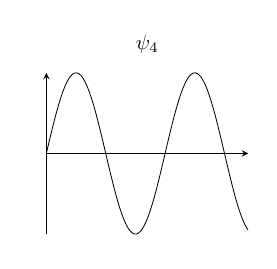
\begin{tikzpicture}[scale=0.75]
\begin{axis}[
    title={\(\psi_4\)},
    axis lines = left,
    axis lines = center,
    xtick style={draw=none},
    ytick style={draw=none},
    xticklabels={},
    yticklabels={},
    xlabel = {},
    ylabel = {},
]

\addplot [
    domain=0:12.566, 
    samples=100, 
    color=black,
]
{sin(deg(0.85*x))};
 
\end{axis}
\end{tikzpicture}
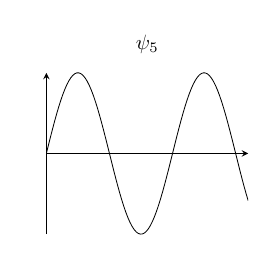
\begin{tikzpicture}[scale=0.75]
\begin{axis}[
    title={\(\psi_5\)},
    axis lines = left,
    axis lines = center,
    xtick style={draw=none},
    ytick style={draw=none},
    xticklabels={},
    yticklabels={},
    xlabel = {},
    ylabel = {},
]

\addplot [
    domain=0:12.566, 
    samples=100, 
    color=black,
]
{sin(deg(0.8*x))};
 
\end{axis}
\end{tikzpicture}
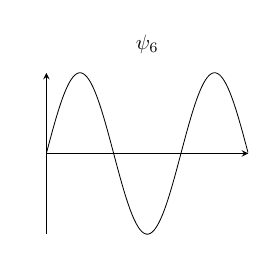
\begin{tikzpicture}[scale=0.75]
\begin{axis}[
    title={\(\psi_6\)},
    axis lines = left,
    axis lines = center,
    xtick style={draw=none},
    ytick style={draw=none},
    xticklabels={},
    yticklabels={},
    xlabel = {},
    ylabel = {},
]

\addplot [
    domain=0:12.566, 
    samples=100, 
    color=black,
]
{sin(deg(0.75*x))};
 
\end{axis}
\end{tikzpicture}
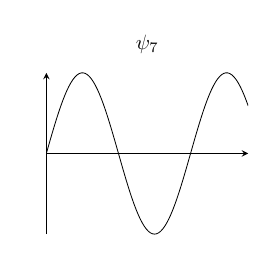
\begin{tikzpicture}[scale=0.75]
\begin{axis}[
    title={\(\psi_7\)},
    axis lines = left,
    axis lines = center,
    xtick style={draw=none},
    ytick style={draw=none},
    xticklabels={},
    yticklabels={},
    xlabel = {},
    ylabel = {},
]

\addplot [
    domain=0:12.566, 
    samples=100, 
    color=black,
]
{sin(deg(0.7*x))};
 
\end{axis}
\end{tikzpicture}
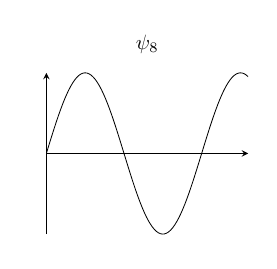
\begin{tikzpicture}[scale=0.75]
\begin{axis}[
    title={\(\psi_8\)},
    axis lines = left,
    axis lines = center,
    xtick style={draw=none},
    ytick style={draw=none},
    xticklabels={},
    yticklabels={},
    xlabel = {},
    ylabel = {},
]

\addplot [
    domain=0:12.566, 
    samples=100, 
    color=black,
]
{sin(deg(0.65*x))};
 
\end{axis}
\end{tikzpicture}
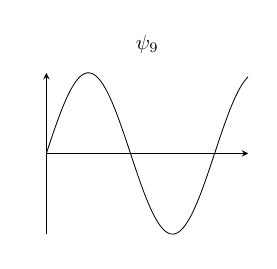
\begin{tikzpicture}[scale=0.75]
\begin{axis}[
    title={\(\psi_9\)},
    axis lines = left,
    axis lines = center,
    xtick style={draw=none},
    ytick style={draw=none},
    xticklabels={},
    yticklabels={},
    xlabel = {},
    ylabel = {},
]

\addplot [
    domain=0:12.566, 
    samples=100, 
    color=black,
]
{sin(deg(0.6*x))};
 
\end{axis}
\end{tikzpicture}
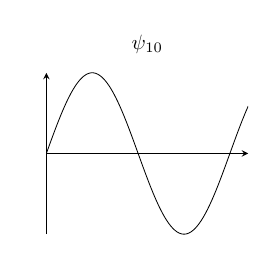
\begin{tikzpicture}[scale=0.75]
\begin{axis}[
    title={\(\psi_{10}\)},
    axis lines = left,
    axis lines = center,
    xtick style={draw=none},
    ytick style={draw=none},
    xticklabels={},
    yticklabels={},
    xlabel = {},
    ylabel = {},
]

\addplot [
    domain=0:12.566, 
    samples=100, 
    color=black,
]
{sin(deg(0.55*x))};
 
\end{axis}
\end{tikzpicture}
\begin{tikzpicture}[scale=0.75]
\begin{axis}[
    title={\(\psi_{11}\)},
    axis lines = left,
    axis lines = center,
    xtick style={draw=none},
    ytick style={draw=none},
    xticklabels={},
    yticklabels={},
    xlabel = {},
    ylabel = {},
]

\addplot [
    domain=0:12.566, 
    samples=100, 
    color=black,
]
{sin(deg(0.5*x))};
 
\end{axis}
\end{tikzpicture}
\begin{tikzpicture}[scale=0.75]
\begin{axis}[
    title={\(\psi_{12}\)},
    axis lines = left,
    axis lines = center,
    xtick style={draw=none},
    ytick style={draw=none},
    xticklabels={},
    yticklabels={},
    xlabel = {},
    ylabel = {},
]

\addplot [
    domain=0:12.566, 
    samples=100, 
    color=black,
]
{sin(deg(0.45*x))};
 
\end{axis}
\end{tikzpicture}
\begin{center}
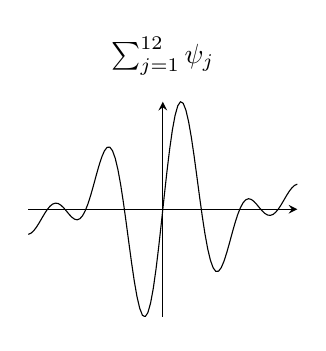
\begin{tikzpicture}[scale=1]
\begin{axis}[
    title={\(\sum_{j=1}^{12}\psi_j\)},
    axis lines = left,
    axis lines = center,
    xtick style={draw=none},
    ytick style={draw=none},
    xticklabels={},
    yticklabels={},
    xlabel = {},
    ylabel = {},
]

\addplot [
    domain=-15.708:15.708, 
    samples=100, 
    color=black,
]
{sin(deg(0.95*x))+sin(deg(0.9*x))+sin(deg(0.85*x))+sin(deg(0.8*x))+sin(deg(0.75*x))+sin(deg(0.7*x))+sin(deg(0.65*x))+sin(deg(0.6*x))+sin(deg(0.55*x))+sin(deg(0.5*x))+sin(deg(0.45*x))};
 
\end{axis}
\end{tikzpicture}
\end{center}

This superposition of different wave frequencies is known as a wave packet. The wave packet is also a solution to the Schr\"odinger equation. The particle isn't equally likely to be anywhere, it is now localised.

Each frequency has an associated wave number \(k_j\). The momentum is \(p=\hb k\) so the momentum is now no longer known precisely. We have an uncertainty of \(\Delta p\). The smaller the wave packet the more localised the particle is and the greater the range of frequencies needed. This gives rise to Heisenberg's uncertainty principle:
\[\Delta x\Delta p_x\ge\frac\hb2\]
Where \(\Delta x\) is uncertainty in position and \(\Delta p_x\) is uncertainty in momentum in the \(x\) direction. This fundamentally limits how well we can measure \(p_x\) and \(x\). A similar relationship between energy and time exists:
\[\Delta E\Delta t\ge\frac\hb2\]

\section{}

If we introduce a potential \(U(x)\) then only certain energies \(E\) are allowed. The energy becomes quantised.

\(\psi_+(x)=Ae^{ikx}\) is a particle moving in the positive \(x\) direction. \(\psi_-(x)=Ae^{-ikx}\) is a particle moving in the negative \(x\) direction. If we sum them together we get a standing wave:
\[\psi=\psi_++\psi_-=Ae^{ikx}+Ae^{-ikx}=A[\cos kx+i\sin kx+\cos kx-i\sin kx]=2A\cos kx\]

A more general solution to the wave equation is given by \(\psi_+=Ae^{i(kx+\varphi)}\):
\[\diff x (Ae^{i(kx+\varphi)})=Aike^{i(kx+\varphi)}\]
\[\diff[2] x(Ae^{i(kx+\varphi)})=-Ak^2e^{i(kx+\varphi)}\]
\[-Ak^2e^{i(kx+\varphi)}+\frac{8\pi^2m}{h^2}[E-u(x)]Ae^{i(kx+\varphi)}=0\]
So given the condition \(k^2=\frac{8\pi^2m}{h^2}\) this is a solution.
The standing wave formed with this solution is:
\[\psi=\psi_++\psi_-=2A\cos(kx+\varphi)=2A\sin\left(kx+\varphi-\frac{\pi}{2}\right)\]
This shows that the standing waves which satisfy the Schr\"odinger equation are sinusoidal.

\subsection*{Infinite square potential}

\begin{center}
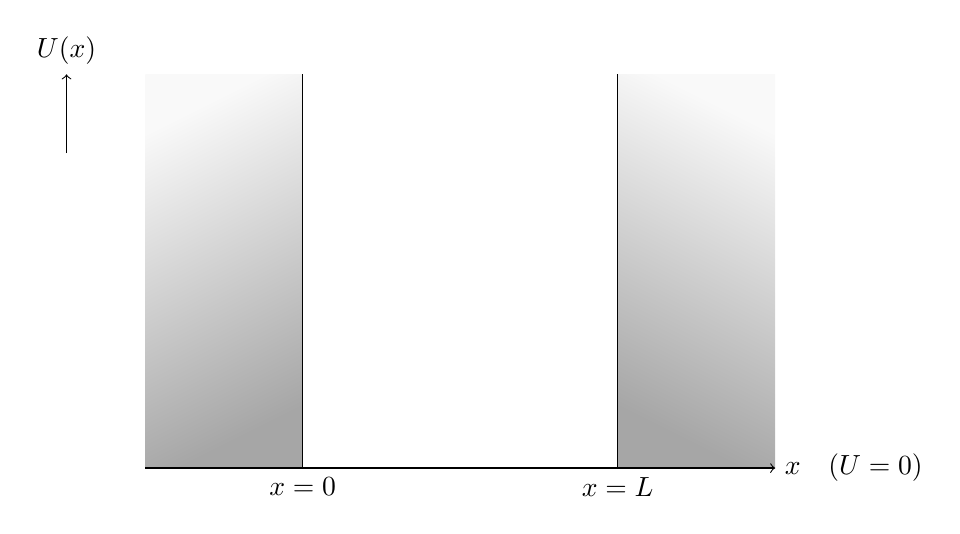
\begin{tikzpicture}
\shade [left color=gray!5, right color=gray!70, shading=axis, shading angle=26.565] (-2,0) -- (-4,0) -- (-4,5) -- (-2,5) -- (-2,0);
\shade [right color=gray!5, left color=gray!70, shading=axis, shading angle=153.435] (2,0) -- (4,0) -- (4,5) -- (2,5) -- (2,0);
\draw [->] (-4,0) -- (4,0);
\draw (-2,0) -- (-2,5);
\draw (2,0) -- (2,5);
\draw [->] (-5,4) -- (-5,5);
\node [below] at (-2,0) {\(x=0\)};
\node [below] at (2,0) {\(x=L\)};
\node [above] at (-5,5) {\(U(x)\)};
\node [right] at (4,0) {\(x\quad (U=0)\)};
\end{tikzpicture}
\end{center}
Now particles can be at \(x\) values outside of the range \(x\in(0,L)\). This means that the probability density function (p.d.f.) is 0 outside of this range:
\[|\psi(0)|^2=|\psi(L)|^2=0\]
\[\implies\psi(0)=\psi(L)=0\]
A standing wave with nodes at \(x=0\) and \(x=L\) is therfore a valid solution to the Scr\"odinger equation in this case:

\begin{center}
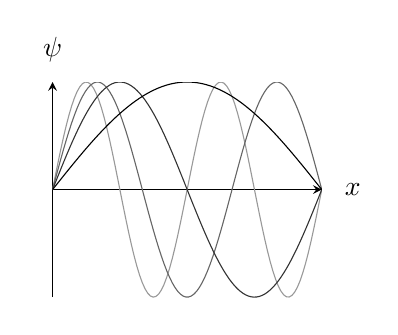
\begin{tikzpicture}[scale=1]
\begin{axis}[
    axis lines = left,
    axis lines = center,
    xtick style={draw=none},
    ytick style={draw=none},
    xticklabels={},
    yticklabels={},
    xlabel = {\(x\)},
    ylabel = {\(\psi\)},
every axis x label/.style={
    at={(ticklabel* cs:1.05)},
    anchor=west,
},
every axis y label/.style={
    at={(ticklabel* cs:1.05)},
    anchor=south,
},
]

\addplot [
    domain=0:3.1415926, 
    samples=100, 
    color=black!40,
]
{sin(deg(4*x))};

\addplot [
    domain=0:3.1415926, 
    samples=100, 
    color=black!60,
]
{sin(deg(3*x))};

\addplot [
    domain=0:3.1415926, 
    samples=100, 
    color=black!80,
]
{sin(deg(2*x))};

\addplot [
    domain=0:3.1415926, 
    samples=100, 
    color=black,
]
{sin(deg(x))};
\end{axis}
\end{tikzpicture}
\end{center}
The solution has wavelength \(\lambda\) which can take the values:
\[\lambda=2L,L,\frac 23L,\frac12L,\cdots\]
Since\(k=\frac{2\pi}{\lambda}\) then \(k\) can take the values:
\[k=\frac{\pi}{L},\frac{2\pi}{L},\frac{3\pi}{L},\frac{4\pi}{L},\cdots=\frac{n\pi}{L}\quad n\in\bb N\]
Here \(n\) is the quantum number \(n=1,2,3,4\cdots\)

In the region between \(x=0\) and \(x=L\) the particle is free so we can use:
\[E=\frac{\hb^2k^2}{2m}=\frac{\hb^2n^2\pi^2}{2mL^2}=\frac{h^2}{8mL^2}n^2\]

\begin{center}
\begin{tikzpicture}
\draw [->] (0,0) -- (0,5);
\node [above] at (0,5) {\(E\)};
\draw (0.5,0.5) -- (5,0.5);
\draw (0.5,2) -- (5,2);
\draw (0.5,4.5) -- (5,4.5);
\node [right] at (5,0.5) {\(\frac{h^2}{8mL^2}\)};
\node [right] at (5,2) {\(4\frac{h^2}{8mL^2}\)};
\node [right] at (5,4.5) {\(9\frac{h^2}{8mL^2}\)};
\end{tikzpicture}
\end{center}
The energy levels are getting further and further appart. Note that the lowest possible energy level is not 0 as \(n\ne0\)

\begin{center}
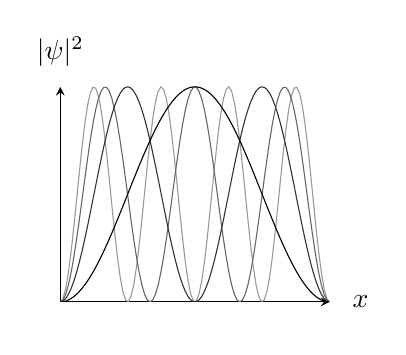
\begin{tikzpicture}[scale=1]
\begin{axis}[
    axis lines = left,
    axis lines = center,
    xtick style={draw=none},
    ytick style={draw=none},
    xticklabels={},
    yticklabels={},
    xlabel = {\(x\)},
    ylabel = {\(|\psi|^2\)},
every axis x label/.style={
    at={(ticklabel* cs:1.05)},
    anchor=west,
},
every axis y label/.style={
    at={(ticklabel* cs:1.05)},
    anchor=south,
},
]

\addplot [
    domain=0:3.1415926, 
    samples=100, 
    color=black!40,
]
{sin(deg(4*x))^2};

\addplot [
    domain=0:3.1415926, 
    samples=100, 
    color=black!60,
]
{sin(deg(3*x))^2};

\addplot [
    domain=0:3.1415926, 
    samples=100, 
    color=black!80,
]
{sin(deg(2*x))^2};

\addplot [
    domain=0:3.1415926, 
    samples=100, 
    color=black,
]
{sin(deg(x))^2};
\end{axis}
\end{tikzpicture}
\end{center}
This shows the p.d.f. for \(n=1,2,3,4\)

We can only measure the probability to find a particle in a region of width \(\Delta x\). To find if the particle is close to \(\frac L2\) we measure the probability to find the particle in \(x\in\left(\frac L2-\frac{\Delta x}{2},\frac L2 + \frac{\Delta x}{2}\right)\)
This means that for \(n=20\) we measure the red line when the p.d.f. looks like the black:

\begin{center}
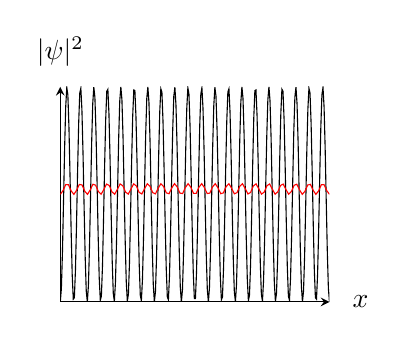
\begin{tikzpicture}
\begin{axis}[
    axis lines = left,
    axis lines = center,
    xtick style={draw=none},
    ytick style={draw=none},
    xticklabels={},
    yticklabels={},
    xlabel = {\(x\)},
    ylabel = {\(|\psi|^2\)},
every axis x label/.style={
    at={(ticklabel* cs:1.05)},
    anchor=west,
},
every axis y label/.style={
    at={(ticklabel* cs:1.05)},
    anchor=south,
},
]

\addplot [
    domain=0:3.1415926, 
    samples=250, 
    color=black,
]
{sin(20*deg(x))^2};

\addplot [
    domain=0:3.1415926, 
    samples=100, 
    color=red,
]
{(1/20)*sin(20*deg(x))^2+(1/2)};

\end{axis}
\end{tikzpicture}
\end{center}
This agrees better with what classical mechanics would predict. This is an example of the correspondance principle:

\begin{displayquote}
For sufficently high quantum numbers the results predicted by quantum mechanics are indistinguishable from the results predicted by classical maechanics.
\end{displayquote}

This can be seen if we consider an airhockey puck on a airhockey table. This idealised system behaves as an infinite square potential. For a puck mass \(m=\SI{50}{g}\), velocity \(v=\SI{5}{m.s^{-1}}\) and a table of length \(L=\SI{2}{m}\) the energy of the puck is given by:
\[E=\frac 12mv^2=\frac 120.05\cdot 5^2=\frac 58\]
\[E_n=\frac{h^2n^2}{8mL^2}\]
\[n=\sqrt{\frac{8mL^2E_n}{h^2}}\]
\[n=\num{1.5e33}\]
\(n\) is very big so quantum predictions will agree with classical predictions.

\section{}

The lowest allowed energy is called the zero-point energy
\[\dv[2]{\psi(x)}{x} + \frac{8\pi^2m}{h^2}[E-U(x)]\psi(x)=0\]

We will consider the potential energy function
\[U(x)=\left\{
\begin{array}{l l}
0 & \text{for } x<L\\
U_1 & \text{for } x\ge L
\end{array}
\right.\]
Where \(U_1>E\). A solution to this is \(\psi(x)=Be^{-\alpha x}\) for \(\alpha\in\bb R\)
\[\dv{\psi}{x}=-\alpha Be^{-\alpha x},\qquad \dv[2]{\psi}{x}=\alpha^2Be^{-\alpha x}\]
\[\alpha^2 B e^{-\alpha x}+\frac{8\pi^2m}{h^2}\underbrace{[E-U_1]}_{<0}Be^{-\alpha x}=0\]
\[\alpha^2 +\frac{8\pi^2m}{h^2}[E-U_1]=0\]
\[\alpha^2=\frac{8\pi^2m}{h^2}\underbrace{[U_1-E]}_{>0}\]
\[\alpha = \sqrt{\frac{8\pi^2m}{h^2}[U_1-E]}\]

So depending on the values of \(\alpha\) and \(x\) \(\psi\) is either increasing or decreasing exponetially in the region where \(x\ge L\). Classicaly the particle wouldn't be allowed in this region but in quantum mechanics it is allowed. In the region where \(U(x) = 0\) \(\psi\) is a standing wave caused by partial reflection at the boundary. In the region where \(U(x) = U_1\) \(\psi\) decays exponetially. Importantly:
\begin{itemize}
\item \(\psi\ne 0\) in the clasicaly forbidden region
\item The wavefunction transitions smoothly at the boundary
\item \(\psi\to0\) as\(x\to\infty\)
\end{itemize}

\subsection*{Harmonic Potential well}

\(U(x)=\frac 12k_{\text{spr}}x^2\) where \(k_{\text{spr}}\) is th espring constant not the wavenumber.

We expect sinusoidal standing waves in the classicaly allowed region and \(\psi\to0\) as \(x\to\pm\infty\)

\(\displaystyle{E_n=\left(n+\frac 12\right)\hb \omega}\) where \(\displaystyle{\omega = \sqrt{\frac{k_{\text{spr}}}{m}}}\) and \(n=0,1,2\dots\)

zero-point energy \(\displaystyle{E_0=\frac 12\hb\omega}\)

This creates evenly spaced energy levels. Inside the clasical boundaries \(\psi\) is a standing wave, outside it decays exponentially.

\subsection*{Quantum tunneling}

If instead we consider a potential
\[U(x) = \left\{
\begin{array}{l l}
0 & \text{for } L_1>x\\
U_1 & \text{for } L_1\le x<L_2\\
0 & \text{for } L_2\le x
\end{array}
\right.\]
Before the increased potential \(\psi\) is a large amplitude standing wave, between \(L_1\) and \(L_2\) \(\psi\) decays exponentially and after \(L_2\) \(\psi\) is a small amplitude standing wave.

\section{}

\subsection*{The Bohr Model of H}

The Bohr model is based on four unjustified postulates:
\begin{itemize}
\item Electrons orbit the nucleus at a fixed radius due to the Coulomb force
\item The angular momentum of the electron is quantised \(l=n\hb\) where \(n=1,2,3,\dots\)
\item The electron doesn't radiate photons when it is in one of these orbits
\item Emission/absorption occurs due to transitions between these orbits
\end{itemize}
Potential energy of an electron in H:
\[PE=U(r)=\frac{q_1q_2}{4\pi\varepsilon_0}=-\frac{e^2}{4\pi\varepsilon_0}\]
Electronstatic and centripetal forces balance:
\[\frac{mv^2}{r}=\frac{e^2}{4\pi\varepsilon_0}\implies KE = \frac 12mv^2=\frac{e^2}{8\pi\varepsilon_0r}\]
Total energy:
\[E=KE+PE=-\frac{e^2}{8\pi\varepsilon_0r}\tag{17.1}\]
The total energy is negative as the electron is bound to the atom and needs to gain energy to leave. Note that \(E\propto\frac 1r\)
\[l=mvr=n\hb\qquad n=1,2,3,\dots\tag{17.2}\]
Balancing forces:
\[\frac{mv^2}{r}=\frac{e^2}{4\pi\varepsilon_0r^2}\tag{17.3}\]
Rearranging (17.1) gives
\[v=\frac{n\hb}{mr}\]
Substituting this into (17.3) gives
\[\frac mr\left(\frac{n\hb}{mr}\right)^2=\frac{e^2}{4\pi\varepsilon_0r^2}\]
\[r=\frac{4\pi\varepsilon_0\hb^2}{me^2}n^2=\underbrace{\frac{\varepsilon_0h^2}{\pi me^2}}_{\text{constant}}n^2\]
Note that \(r\propto n^2\)

The smalles possible radius occurs at \(n=1\):
\[r_1=\frac{\varepsilon_0h^2}{\pi me^2}=\SI{5.29e-11}{m}=a\]
\(a\) is the Bohr radius. If we substitute this into (17.1) we get
\[E=-\frac{m^2e^4}{8\varepsilon_0^2h^2n^2}=-\frac{13.6}{n^2}\mskip3mu\si{eV}\]

\subsection*{Quantum Model}

The Bohr model misses several predictions that the quantum model sucssesfully makes. The quantum model comes from solving the 3D time invariant Schr\"odinger equation for \(\psi(x,y,z)\)
\[\pd[2]{\psi}{x}+\pd[2]{\psi}{y}+\pd[2]{\psi}{z}++\frac{8\pi^2m}{h^2}[E-U(x,y,z)]\psi=0\]
\[U(x,y,z)=-\frac{e^2}{4\pi\varepsilon_0r}\quad\text{where}\quad r=\sqrt{x^2+y^2+z^2}\]
Using spherical polar coordinates \((r,\vartheta,\varphi)\), as the system is sphericaly symmetrical, the solution can be written as a product of functions dependant on quantum numbers \(n,l\) and \(m_l\)
\[\psi(r,\vartheta,\varphi)=R_{n,l}(r)\Theta_{l,m_l}(\vartheta)\Phi_{m_l}(\varphi)\]
This gives
\[E_n=-\frac{m^2e^4}{8\varepsilon_0^2h^2n^2}=-\frac{13.6}{n^2}\mskip3mu\si{eV}\]

\section{}

\begin{center}
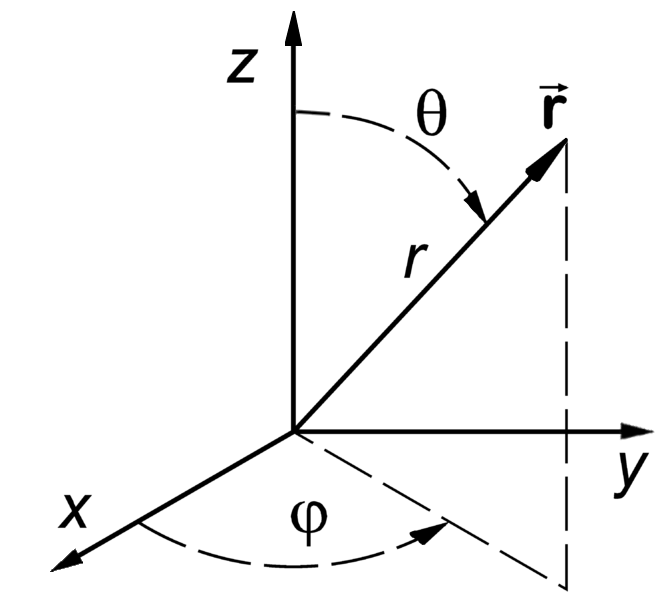
\includegraphics[scale = 0.2]{SphericalPolarCoordinates}
\end{center}


We have to apply boundary conditions for the 3D Schr\"odinger equation that \(\psi\to0\) as \(x,y,z\to\infty\)

\(n\) is the principal quantum number. It determines the energy and radial extent of the wave function.

\(n=1,2,3,\dots\) \(n\in\bb N\)

\(l\) is the orbital angular momentum quantum number. It determines the magnitude of angular momentum.

\(l=1,2,\dots,n-1\) \(l\in\bb N\) and \(l<n\)

\(m_l\) is the magnetic quantum number. It determines the direction of angular momentum.

\(m_l=-l,-l+1,\dots,0,\dots l-1,l\) \(m_l\in\bb Z\) and \(|m_l|\le l\)

Suppose that \(n=2\), this means that \(l\) can take two values, 0 or 1. When \(l=0\) \(m_l=1\), when \(l=1\) \(m_l=-1,0,1\).

The angular momentum is given by \(|\vv L|=\sqrt{l(l+1)}\hb\). For \(l=1\) this means the angular momentum is \(|\vv L|=\sqrt{2}\hb\). Using \(m_l\) we can measure the components of \(\vv L\) in a direction. By convention we measure it for the \(z\) direction \(L_z=m_l\hb\). This gives us possible anugular momentums \(\vv L\) as shown in the diagram

\begin{center}
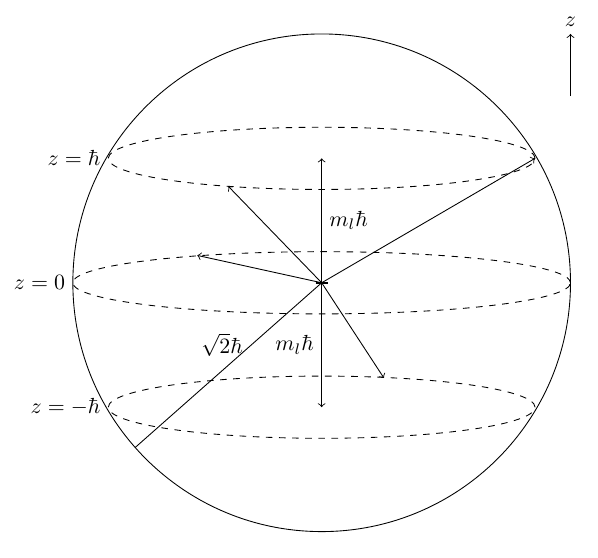
\includegraphics[scale=0.4]{ElectronAngularMomentum}
\end{center}
This shows some of the possible angular momentum vectors \(\vv L\) for \(n=2\). The vectors are all from the origin to some point on the three dotted circles which lie in the planes \(z=-\hb,\,z=0\) and \(z=\hb\). The radius of the sphere is \(\sqrt 2\hb\).

If we proceed to measure a different component of the angular momentum we no longer know the component in the previously measured direction.

For \(n=1\)
\[R_{n=1}(r)=\frac{1}{\sqrt\pi a^{\frac32}}e^{-\frac ra}\]
Where \(a=\num{5.3e-11}\) is the Bohr radius

For a randomly chosen point in space the probability of it being a given distance \(r\) from the origin is proportional to the surface area of the sphere radius \(r\) which is \(4\pi r^2\)

When using \(\psi(r)\) instead of \(\psi(x\) the radial probability density is
\[P(r)=4\pi r^2|\psi(r)|^2\]
For \(n=1\)
\[P_{n=1}(r)=4\pi r^2[R_{n=1}(r)]^2=\frac{4}{a^3}r^2e^{-2ra}\]

\begin{center}
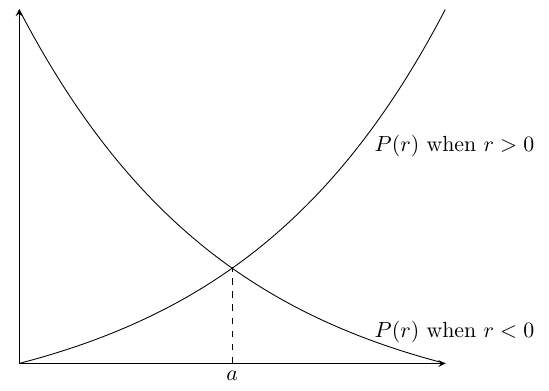
\includegraphics[scale=0.4]{RadialProbabilityDistribution}
\end{center}
The most likely radial distance is \(a\).

This gives rise to the orbitals. Each orbital is denoted by \(n\) and a letter representing \(l\):

\begin{center}
\begin{tabular}{|c|cccccc|}\hline
\(l\) & 0 & 1 & 2 & 3 & 4 & 5\\\hline
letter& s & p & d & f & g & h\\\hline
\end{tabular}
\end{center}
For example 1s is \(n=1,\,l=0\) and 3d is \(n=3,\,l=2\)


\section{}

Electrons also have spin quantum numbers \(s\) and \(m_s\). SPin is predicted when relativity is added to quantum mechanics. The magnitude of total spin \(|\vv S|\) is given by
\[|\vv S|=\sqrt{s(s+1)}\hb\]
The component of spin in the \(z\) direction is given by
\[S_z=m_s\hb\]
For electrons \(s=\frac12\). \(m_2\in\{-s,-s+1,\dots ,s-1,s\}\) so for an electron \(m_s=\pm\frac12\). Electrons are described by the four quantum numbers \(n,l,m_l\) and \(m_s\).
\[|\vv S|=\sqrt{s(s+1)}\hb=\frac{\sqrt{3}}{2}\]
\[S_z=m_s\hb=\pm\frac12\hb\]
For hydrogen the Schr\''odinger equation can be solved exactly. For multi-electron systems all of the electrons repel eachother. This means it isn't possible to solve the Schr\''odinger equation exactly, however, numerical solutions can be found. In multi-electron systems the electrons may have the same quantum numbers as a single electron system but the energies will be different. In a multi-electron system the energy depends mostly on \(n\) and \(l\).

The Pauli exclusion principal states

\begin{displayquote}
No two fermions in a system may have the same quantum state
\end{displayquote}

A fermion is any particle with \(s=\frac{2m+1}{2}\) for \(m\in\bb Z\). This includes electrons, protons, neutrons, muons and neutrinos. Particles with \(s=m\) for \(m\in\bb Z\). This includes photons, the Higg's boson and \(^2\)He.

Spin up is used to refer to \(s=\frac12\) and spin down refers to \(s=-\frac12\).

A consequence of the Pauli exclusion principal is that each orbital can hold two electrons for each value of \(l\) (spin up and spin down). This means that each s orbital can hold two electrons, p orbitals can hold 6 , d orbitals can hold 10 and f orbitals can hold 14.

The probability per unit time of a transition between energy levels is not the same for all transitions. If \(\Delta l=1\) the transition is likely to occur and is said to be an allowed transition. If an electron can deexcite by such a transition it will and quickly. If \(\Delta l\ne 1\) then the transition is less likely and is said to be ``forbiden'' (but can still occur). If there are no other transitions possible an electron will deexcite by this transition but it will take a long time.

Flourescence is emission of light during illumination as the light excites electrons which then fall back to the ground state in several lower frequency stages emitting multiple photon along the way.

Phosphorecence is emission of light after illumination as the light excites electrons into forbiden transitions which then don't fall back to ground state for a long time, possibly after the illumination has been removed.

\section{}

Fast (allowed) transitions have small \(\Delta t\) and therefore large error in their energy \(\Delta E\).

Slow (forbidden) transitions have large \(\Delta t\) and therefore small error in their energy \(\Delta E\).

\(hf=E_1-E_2\) has some variance since \(\Delta E\ne 0\). THis means we don't get one frequency \(f\) but a range of frequencies. This means instead of a sharp line we get a brad line. The range of frequencies is known as the line width.

\subsection*{Induced emission}

\begin{center}
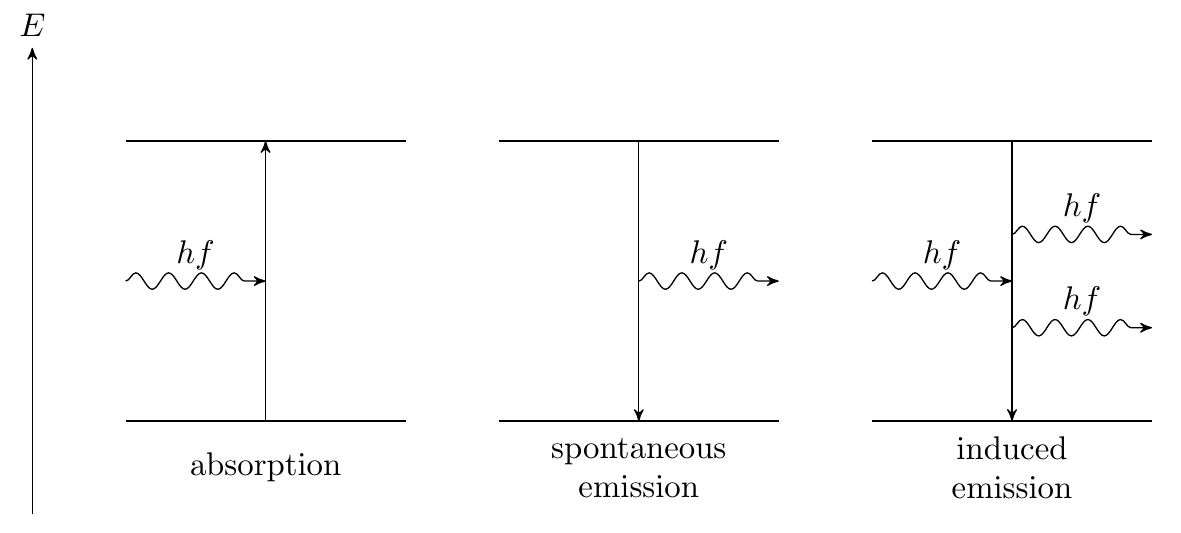
\includegraphics[scale=0.3]{EmissionAbsorptionTypes}
\end{center}
Induced (stimulated) emission ocurs when an electron can only decay by a forbidden transistion. A photon energy \(hf=E_1-E_0\) will induce the electron to decay and emit two photons both with energy \(hf\) in identical quantum states.

\(N_0\) is the number of atoms in ground state \(E_0\)

\(N_1\) is the number of atoms in excited state \(E_1\)

If we introduce a photon \(hf=E_1-E_0\)
\begin{itemize}
\item if \(N_0>N_1\) absorption is more likely
\item if \(N_1>N_0\) induced emission is more
\end{itemize}
So for stimulated emission to occur on a large scale we need \(N_1>N_0\) When this is true the number of photons increases. This is called photon amplification.

\subsection*{Boltzmann Distribution}

The Boltzmann distribution is that when in thermal equilibrium the ratio of \(N_1\) and \(N_0\) is
\[\frac{N_1}{N_0}=e^{-\frac{\Delta E}{kT}}\]
Where \(\Delta E=E_1-E_0\), \(k\) is the Boltzmann constant \(k=\num{1.38e-23}\,\si{J.K^{-1}}\) and \(T\) is the temperature in \(K\).

For a simple two level energy system \(\frac{N_1}{N_0}<1\,\A \Delta E\). However for photon amplification we want \(\frac{N_1}{N_0}>1\). This is possible in a three or more energy level system. The electrons are excited to the highest energy level from the ground state by the ``pump''. They quickly decay to a middle energy level by an allowed transition and they collect here until \(N_1>N_0\) where they decay by stimulated emission down a forbidden energy level.

\begin{center}
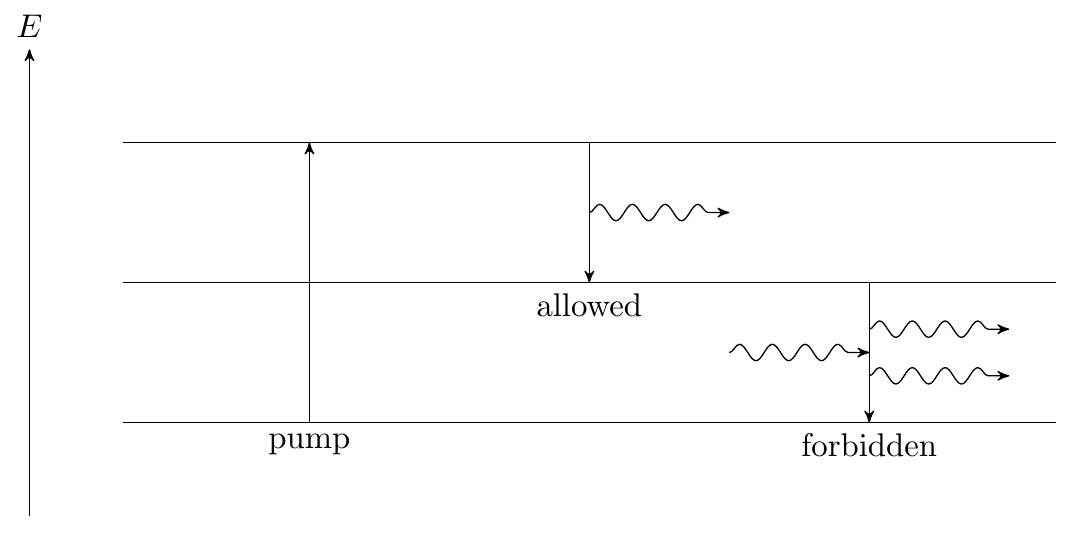
\includegraphics[scale=0.3]{LasingEnergyLevels}
\end{center}

The pump can be other photons of a higher energy, electricity, heat or any other energy source. The pump stage is very quick so atoms are moved out of the ground state quickly.

In this case the forbidden transition is called the lasing transition.

Efficency can be improved by surrounding the material being used to emit light in mirrors with a semi silvered mirror where we want the light to leave. This increases efficency by reflecting back photons of necessary energy to create more stimulated electrons and perpetuate the photon amplification.

\section{}

Electrons are responsible for bonding. Generally the highest energy (highest \(n\) and \(l\)) electrons take part in bonding. THe electrons arrange to get the lowest possible energy. In a covalent bond electrons are shared and both nuclei are attracted to the elctrons. In an ionic bond electrons are donoted from one atom and accepeted by another leading to a difference in charge and hence electrostatic attraction. A shell of electrons is all electrons with the same value of \(n\). A subshell of electrons is all the electorns with the same values of \(n\) and\(l\). 

\subsection*{Formation of H\(_2\)}

As the hydrogen nuclei come together the electrostatic potentials overlap lowering the energy of each energy level. Eventually the pdfs of the electrons overlap and the most likely place to find the electrons is between the two nuclei and the electrons can move between the two atoms. The energy to seperate the two nuclei is approximately \SI{4.5}{eV} which is a lot less than the ionisation energy of the electrons \SI{13.6}{eV}. In general it is much easier to break bonds than to ionise an atom.

\subsection*{Ionic Bonding}

\[\text{\ce{Na}}(\mathrm{Z}=11)\mathrm{1s^22s^22p^63s^1}\ce{->Na+}\mathrm{1s^22s^22p^6}\]
\[\text{\ce{Cl}}(\mathrm{Z}=17)\mathrm{1s^22s^22p^63s^23p^5}\ce{->Cl-}\mathrm{1s^22s^22p^63s^23p^6}\]
Both have full valence shells. This arrangement is lower energy as \ce{Na} goes from 3s energy to 2p energy and \ce{Cl} stays at 3p energy.

\subsection*{Properties}
Typical properties of ionic and covalent substances at stp
\begin{center}
\begin{tabular}{|c|cc|}\hline
 Property & Ionic & Covalent\\ \hline
 Phase & Solid & Gas\\
 Density & High & Low\\
 Melting point & High & Low\\
 Boiling point & High & Low\\
 Electrical properties & Conducts when molten/in solution & Insulator\\\hline
\end{tabular}
\end{center}

Resistivity is an intrinsic property of a material. It is related to resistance \(R\)
\[R=\rho\frac{L}{A}\]
Where \(L\) is lenght and \(A\) is cross sectional area. The units of resistivity are \si{\ohm m}. Conductors have a low resestivity \((\rho\approx\SI{e-8}{\ohm m})\) and insulators have relatively high resistivity \((\rho\approx\SI{e17}{\ohm m})\). Resistivity isn't constant with temperature. We quantify how resistivity changes  by \(\alpha\) the temperature coefficent of resistivity
\[\alpha=\frac{1}{\rho}\dv{\rho}{T}\]
Where \(T\) is the temperature in \si{K}. The units of \(\alpha\) are \si{K^{-1}}. The larger \(\alpha\) is the more resistivity changes with respect to temperature. This gives us the approximation \(\Delta\rho=\alpha\Delta T\rho\)

%\documentclass{article}
%\usepackage{amsmath
%                   ,siunitx
%                   ,fancyhdr
%                   ,amssymb
%                   ,centernot
%                   %,tikz
%                   %,tikzsymbols
%                   %,pgfplots
%                   ,graphicx
%                   ,csquotes
%                   ,bm
%                   ,tocloft
%                   ,titlesec
%                   ,parskip
%                   ,leftidx
%                   ,hyperref}
%\usepackage[margin=1in]{geometry}
%\usepackage[version=4]{mhchem}
%
%\cftsetindents{section}{0.75em}{6em}
%\renewcommand{\cftsecpresnum}{Lecture }  % Sets up the table of contents and section heading
%\renewcommand{\cftdot}{.}
%\renewcommand{\cftsecleader}{\cftdotfill{\cftdotsep}}
%\titlelabel{Lecture \thetitle}
%\setcounter{section}{0}
%
%%\pgfplotsset{width=5cm,compat=1.9}  % sets version and standard width for pgfplots, I just copied values from the internet
%\graphicspath{ {./Images/} }  % Tells graphicx where images are stored relative to this document
%\hypersetup{hidelinks}  % makes links invisible in table of contents
%
%\newcommand{\vh}[1]{\vec{\hat{#1}}}
%%\renewcommand{\vec}[1]{\underline{#1}}
%\renewcommand{\vec}[1]{\bm{#1}}
%\newcommand{\vv}[1]{\vec{#1}}
%\newcommand{\ve}[1]{\vec{\hat{e}_{#1}}}
%\newcommand{\pd}[3][]{\frac{\partial^{#1}{#2}}{\partial{#3}^{#1}}}
%\newcommand{\dv}[3][]{\frac{d^{#1}{#2}}{d{#3}^{#1}}}
%\newcommand{\pdiff}[2][]{\frac{\partial^{#1}}{\partial{#2}^{#1}}}
%\newcommand{\diff}[2][]{\frac{d^{#1}}{d{#2}^{#1}}}
%\newcommand{\A}{\forall\,}
%\newcommand{\E}{\exists\,}
%\newcommand{\bb}[1]{\mathbb{#1}}
%\newcommand{\cc}[1]{\overline{#1}}
%\newcommand{\hb}{\hbar}
%
%%%%%%%%%%%%%%%%%%%%%%%%%%%%%%%%%%%%%%%%%
%% Copy these commands to the complete document:
%\newcommand{\aparticle}{\ensuremath{\alpha} particle}
%\newcommand{\aparticles}{\ensuremath{\alpha} particles}
%\newcommand{\bparticle}{\ensuremath{\beta} particle}
%\newcommand{\bparticles}{\ensuremath{\beta} particles}
%\newcommand{\bpparticle}{\ensuremath{\beta^+} particle}
%\newcommand{\bmparticle}{\ensuremath{\beta^-} particle}
%\newcommand{\proton}{\ensuremath{\mathrm{p}}}
%\newcommand{\neutron}{\ensuremath{\mathrm{n}}}
%\newcommand{\electron}{\ensuremath{\mathrm{e}^-}}
%\newcommand{\positron}{\ensuremath{\mathrm{e}^+}}
%\newcommand{\neutrino}[1][]{\ensuremath{\nu_{#1}}}
%\newcommand{\antineutrino}[1][]{\ensuremath{\bar\nu_{#1}}}
%\newcommand{\muonm}{\ensuremath{\mu^-}}
%\newcommand{\muonp}{\ensuremath{\mu^+}}
%\newcommand{\tauonm}{\ensuremath{\tau^-}}
%\newcommand{\tauonp}{\ensuremath{\tau^+}}
%\newcommand{\piplus}{\ensuremath{\pi^+}}
%\newcommand{\piminus}{\ensuremath{\pi^-}}
%\newcommand{\pizero}{\ensuremath{\pi^0}}
%\newcommand{\kplus}{\ensuremath{\mathrm{k^+}}}
%\newcommand{\kminus}{\ensuremath{\mathrm{k^-}}}
%\newcommand{\kzero}{\ensuremath{\mathrm{k^0}}}
%\newcommand{\antikzero}{\ensuremath{\mathrm{\bar k^0}}}
%\newcommand{\up}{\ensuremath{\mathrm{u}}}
%\newcommand{\down}{\ensuremath{\mathrm{d}}}
%\newcommand{\charm}{\ensuremath{\mathrm{c}}}
%\newcommand{\strange}{\ensuremath{\mathrm{s}}}
%\newcommand{\topquark}{\ensuremath{\mathrm{t}}}
%\newcommand{\bottom}{\ensuremath{\mathrm{b}}}
%\newcommand{\quark}{\ensuremath{\mathrm{q}}}
%\newcommand{\antiquark}{\ensuremath{\mathrm{\bar q}}}
%\newcommand{\red}{\ensuremath{\mathrm{r}}}
%\newcommand{\green}{\ensuremath{\mathrm{g}}}
%\newcommand{\blue}{\ensuremath{\mathrm{b}}}
%\newcommand{\wplus}{\ensuremath{\mathrm{W^+}}}
%\newcommand{\wminus}{\ensuremath{\mathrm{W^-}}}
%\newcommand{\wpm}{\ensuremath{\mathrm{W^\pm}}}
%\newcommand{\zboson}{\ensuremath{\mathrm{Z^0}}}
%
%\DeclareSIUnit{\solarmass}{\ensuremath{\mathrm{M_\odot}}}
%%%%%%%%%%%%%%%%%%%%%%%%%%%%%%%%%%%%%%%%%
%
%
%\newcounter{example}[section]
%\newenvironment{example}[1][]{\refstepcounter{example}\vspace{-0.2cm}
%\subsubsection*{Example~\thesection.\theexample} \rmfamily}{\par}
%
%%The stuff below sets up header/footer and shrinks margins
%\pagestyle{fancy}
%\lhead{Willoughby Seago}
%\rhead{Physics 1B lecture notes}
%\cfoot{Page \thepage}
%\renewcommand{\headrulewidth}{0.4pt}
%\renewcommand{\footrulewidth}{0.4pt}
%\setlength{\parindent}{0pt}
%
%%The stuff below is used to set up the title
%\title{Physics 1B Lecture Notes}
%\author{Willoughby Seago}
%\date{18 January 2019}
%
%\begin{document}
\part{Nuclear, Particle and Astro Physics}
\section{}

\SI{1}{eV} is the energy gained when one electron is accelerated through a potential difference of \SI{1}{V}.\linebreak \SI{1}{eV}=\num{1.6e-19}\,\si{J}. Using energy-mass equivalency it is possible to write mass as \(m=E/c^2\). This means that \si{MeV/c^{2}} is a unit of mass. Another unit of mass is the atomic mass unit \si{u}, which is defined as \(1/12\) the mass of \ce{^12_6C}.

\begin{center}
\begin{tabular}{cccc}\hline
 & Mass in \si{kg} & Mass in \si{eV/c^2} & Mass in \si{u} \\\hline
Proton & \num{1.673e-27}\,\si{kg} & \SI{938.3}{MeV/c^2} & \SI{1.007}{u}\\
Neutron & \num{1.675e-27}\,\si{kg} & \SI{939.6}{MeV/c^2} & \SI{1.009}{u}\\
Electron & \num{9.11e-31}\,\si{kg} & \SI{511}{KeV/c^2} & \SI{0.0005}{u}\\
\SI{1}{kg} & \SI{1}{kg} & \num{5.61e35}\,\si{eV/c^2} & \num{6.022e26}\,\si{u}\\
\SI{1}{MeV/c^2} & \num{1.78e-30}\,\si{kg} & \SI{1}{MeV/c^2} & \SI{0.0011}{u}\\
\SI{1}{u} & \num{1.66e-27}{kg} & \SI{931.49}{MeV/c^2} & \SI{1}{u}\\\hline
\end{tabular}
\end{center}

In 1897 electrons were discovered and JJ Thompson developed the plum pudding model. In 1908 Geiger and Marsden (supervised by Rutherford) discovered that the mass was concentrated at the center of the atom.

\begin{example}
An \(\alpha\) particle has mass \(\approx\SI{4000}{MeV/c^2}\) and kinetic energy \(\approx\SI{5}{MeV}\). What is the \(\alpha\) particle's velocity?

\(E\ll m/c^2\) so it is non-relativistic.
\[E=\frac12mv^2\implies\SI{5}{MeV}=\frac12(\SI{4000}{MeV/c^2})v^2\]
\[\frac{\SI{10}{MeV}}{\SI{4000}{MeV}}=\frac{v^2}{\si{c^2}}\]
\[\frac{v^2}{\si{c^2}}=\frac{1}{400}\]
\[v=\frac{\si{c}}{20}=\SI{15000}{km s^{-1}}\]
A good check to do now is that \(v\ll c\) so it is definitely non-relativistic.
\end{example}
\begin{example}
What energy electron do you need to probe a proton?

A photon has a diameter of approximately \SI{1}{fm}, so we need electrons with wavelength of the same size.

\[p=\frac{h}{\lambda},\qquad\lambda\approx\SI{1}{fm}\]
\[p=\num{6.63e-19}\,\si{Js/m}=\SI{4.14}{eVs/m}\]
\[c=\num{3e8}\,\si{m/s}\implies\si{s/m}=\num{3e8}\,\si{/c}\]
\[p=\num{1.23e9}\,\si{eV/c}=\SI{1.23}{GeV/c}\]
\[E^2=p^2\mathrm{c}^2+m_0^2c^4\]
\[p=\SI{1.23}{GeV/c}\implies p^2c^2=(\SI{1.23}{GeV})^2\]
\[m_0=\SI{511}{keV/c^2}\implies m_0^2c^4=(\SI{511}{keV})^2\]
\[E^2=(\SI{1.23}{GeV})^2+(\SI{511}{keV})^2=\SI{1.23}{GeV^2}\]
So when \(E\gg m\) we get \(E=pc\) just as it does for a photon. Hence the energy required to probe a proton is \(\SI{1.11}{GeV}\).
\end{example}

\section{}

Nuclei are described by two numbers, the atomic number \(Z\), which is the number of protons, and the atomic mass \(A\) which is the number of nucleons. The number of neutrons is \(N=A-Z\). The radius of an average atom is \(10^{-10}\,\si{m}\). The radius of a nucleon is \(\approx\SI{1}{fm}=10^{-15}\,\si{m}\). Nuclear volume is proportional to the radius cubed, which is proportional to the number of nucleons. This results in a nuclear radius given by \(\num{1.2e-15}A^{1/3}\,\si{m}\).

The mass of an atom is less than the sum of the mass of its constituent parts. This mass difference results in the binding energy of the nucleus. If the mass of the nucleus is \(M(A,Z)\), then the binding energy \(BE\) is given by
\[BE=[Zm_p+(A-Z)m_n-M(A,Z)]c^2\]
The graph below shows the nuclear binding energy per nucleon

\begin{center}
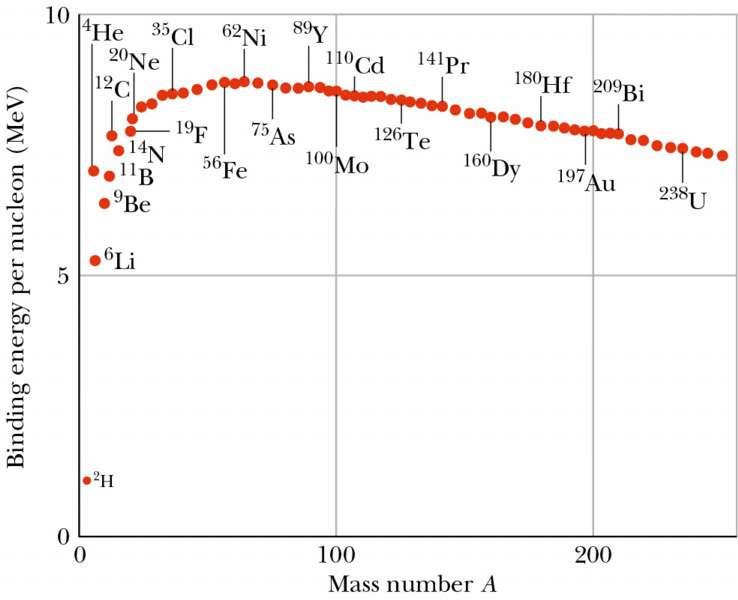
\includegraphics{BindingEnergyPerNucleon}
\end{center}

The graph peaks at \ce{^56Fe}. This is the most stable isotope. Isotopes to the left of \ce{^56Fe} relase energy by fusion. Isotopes to the right of \ce{^56Fe} release energy by fission.

The force that binds the nucleons is the strong force. The graph below shows the nucleon-nucleon potential \(U(r)\) and the magnitude of the force is given by \(F=-\dv Ur\). It can be seen that the strong force is repulsive under about \SI{1}{fm} and attractive from \SI{1}{fm} to about \SI{3}{fm} and beyond \SI{3}{fm} has little or no effect.

\begin{center}
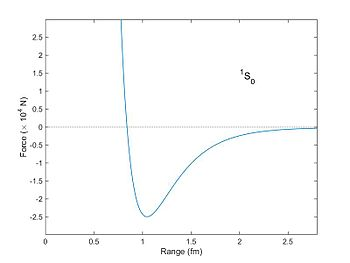
\includegraphics[scale=0.5]{StrongForce}
\end{center}

The most widely accepted model for how forces are mediated is that virtual particles are exchanged, this means that particles are created and travel between other particles carrying momentum and charge. This is allowed as long as \(\Delta E\Delta t\ge\hb/2\).

\begin{example}
A force is mediated by the exchange of virtual pions of mass \SI{140}{MeV/c^2}. How long can these particles exist for (ignoring relativistic effects)?

\begin{align*}
\Delta E\Delta t&>\hb\\
\Delta t&>\frac{\hb}{\SI{140}{MeV/c^2}}\\
\Delta t&>\frac{\num{1.05e-34}\,\si{Js}}{\num{140e6}\cdot\num{1.6e-19}\,\si{J}}\\
\Delta t&>\num{4.7e-34}\,\si{s}
\end{align*}
\end{example}

\section{}

\subsection*{Alpha Decay}

An \aparticle is a \ce{_2^4He} nucleus. \(\alpha\) decay happens when a large, unstable nucleus breaks into a smaller, more stable nucleus and an \aparticle, as in the example below:
\[\leftidx{_Z^A}{X}{}\ce{->}\leftidx{_{Z-4}^{A-2}}{X'}{}+\alpha\]
\subsubsection*{Conserved Quantities}
\begin{itemize}
\item Number of protons
\item Number of neutrons
\item Charge
\item Energy
\begin{itemize}
\item Mass before is larger than the mass after
\item Excess mass is turned into kinetic energy
\item Both the \aparticle and daughter nucleus have the same magnitude of momentum
\item The kinetic energy and velocity of the \aparticle are greater than the daughter nucleus'
\end{itemize}
\end{itemize}

Within \SI{1}{fm} of the nucleus the \aparticle is bound to the nucleus, outside of this distance the potential is very high and then decreases exponentialy. For \(\alpha\) decay the \aparticle must quantum tunnel through this energy barrier. Outside of the range of the strong force the potential is given by
\[U=\frac{1}{4\pi\varepsilon_0}\frac{Z_1Z_2}{r}\]
 Inside the barrier the \aparticle has ``negative energy''. This just means that there is something weird with complex numbers going on here.
 
The \aparticle has a charge of +2 so it interacts a lot with matter. This means that \aparticles are stopped by skin or paper.

\(\alpha\) decay is due to the strong force.

\subsection*{Beta Decay}

A \bmparticle is an electron and a \bmparticle is a positron. The decay occuring with \(\beta^-\) decay is
\[\leftidx{^Z_A}{\mathrm{X}}{}\ce{->}\leftidx{_{\hphantom{{}+1}A}^{Z+1}}{\mathrm{X}'}{}+\electron+\antineutrino[e]\]
\[\neutron\ce{->}\proton+\electron+\antineutrino[e]\]

\(\beta^+\) decay:
\[\leftidx{^Z_A}{\mathrm{X}}{}\ce{->}\leftidx{_{\hphantom{{}-1}A}^{Z-1}}{\mathrm{X}'}{}+\positron+\neutrino[e]\]
\[\proton\ce{->}\neutron+\positron+\neutrino[e]\]

Electron capture:
\[\leftidx{^Z_A}{\mathrm{X}}{}+\electron\ce{->}\leftidx{^{Z-1}_{\hphantom{{}-1}A}}{\mathrm{X}'}{}+\neutrino[e]\]
\[\proton+\electron\ce{->}\neutron+\neutrino[e]\]

\bparticles are less massive and have a lower magnitude of charge than \aparticles. This means that they interact with matter less. Consequently they need a few milimeters of aluminium to stop them.

\subsection*{Gamma Decay}

\begin{center}
\begin{tabular}{c|ccc}
Part of the spectrum & Visible & x-rays & gamma rays\\\hline
Typical energy measured in & \si{eV}& \si{keV} & \si{MeV}
\end{tabular}
\end{center}

Like electrons, nuclei also have excited states but since the radius is much less than for an atom the energy of these excited states is much greater. This means that decays of nuclei to ground states tend to have energies in the \si{MeV}s so they are in the gamma ray part of the spectrum. To stop a gamma ray a few inches of lead are needed.

\section{}

\subsection*{Spontaneous Fission}

Spontaneous fission occurs when a heavy, unstable nucleus splits into two smaller, individualy more stable nuclei. Typicaly the two daughter nuclei aren't the same mass. Often neutrons are produced at the same time. This is a slow process.

\subsection*{Induced Fission}

A neutron is fired at \ce{^235U} which makes \ce{^236U} which has a very short half life and quickly decays into two daughter nuclei and some neutrons. The number of neutrons produced depends on the daughter nuclei produced. If on average more than one neutron is produced then a chain reaction will occur. Typically \SI{200}{MeV} of energy is released per fission event. This corresponds to about \SI{0.2}{u} of mass being converted to energy. A \SI{1}{GW} power station requires about \SI{1}{g} of mass to be converted to energy per day which means approximately \SI{1.2}{kg} of \ce{^235} is used per day.

\subsection*{Fusion}

The most common fusion reaction on earth is deuterium (\ce{D}/\ce{^2H}) and tritium (\ce{T}/\ce{^3H}). This results in the reaction below
\[\mathrm{T+D}\ce{->^4He}+\neutron\]
This reaction releases \SI{17.6}{MeV} of energy. This is known as D--T fusion.  What actually occurs is that \ce{^5He} is produced but because its half life is less than \(10^{-15}\,\si{s}\) it immediately falls apart into \ce{^4He} and a neutron. The mass of the LHS of the reaction is about \SI{5.03}{u} and the mass of the RHS is about \SI{5.01}{u}. This means \SI{0.02}{u} of mass is converted to energy.

Fusion also occurs in the sun. The most common process at this stage in the suns life is
\begin{align*}
\ce{^1H}+\ce{^1H}&\ce{->}\ce{^2H} & (\text{Slow})\\
\ce{^1H}+\ce{^2H}&\ce{->}\ce{^3He} & (\text{Fast})\\
\ce{^3He}+\ce{^3He}&\ce{->}\ce{^4He}+2\ce{^1H} & (\text{Fast})
\end{align*}
The first step is the rate determining step. This reaction takes about 1 billion years. The sun is the equivalent of 100 billion nuclear bombs per second. Every second the sun converts \SI{655}{Mton} of hydrogen to \SI{650}{Mton} of helium.

In bigger stars another common cycle is the CNO cycle where several isotopes of carbon, nitrogen and oxygen are produced along with other smaller particles. It cycles around and ends up with energy being released but the same elements being present.

\subsection*{Particle Physics}

\begin{center}
\begin{tabular}{ccc}\hline
Particle & Size (\si{m}) & Relative size\\\hline
Atom & \(10^{-10}\) & 1\\[0.2em]
Nuclei & \(10^{-14}\) & \(\frac{1}{10000}\)\\[0.2em]
Nucleon & \(10^{-15}\) & \(\frac{1}{100000}\)\\[0.2em]
Quarks/leptons & \(<10^{-18}\) & \(<\frac{1}{100000000}\)\\\hline
\end{tabular}
\end{center}

We believe quarks and leptons are ``point like'' and have no substructure. We can't get individual quarks by themselves due to quark confinement. We have to defer that quarks exist from their influence on measurements such as scattering, decays and bound systems.

To measure small scales we need very large energies. From c. 1910 we have used cosmic rays and radioactive decays for this, from c. 1940 we have also used particle accelerators. Originally cloud chambers were used to detect these particles. Now more sensitive equipment such as ATLAS and CMS is used.

\section{}

Dirac proposed a new equation which took into account quantum mechanics and special relativity. This gave the energy of a particle as
\[E^2=p^2c^2+m^2c^4\]
\[E=\pm\sqrt{p^2c^2+m^2c^4}\]
If \(E>0\) then this is an ordinary particle. The negative energy gave rise to the possibility of antiparticles which were later shown to exist. This shows that every particle has a corresponding antiparticle. To the best of our knowledge antiparticles act just like particles traveling backwards in time.

Positrons (antielectrons) were discovered when a path in a cloud chamber in a magnetic field had equal radius of curvature (therefore momentum and mass) but opposite direction of curvature to the paths known to be caused by electrons. This could only happen if the positron had opposite charge to the electron since the curvature in a magnetic field is described by
\[\vv F=q(\vv E+\vv v\times\vv B)\]

The muon was discovered as it had a much larger radius of curvature (so less curvature) than an electron but was in the same direction (so a muon is negative). The mass of a muon is approximately 200 times the mass of an electron. Muons don't react strongly with protons but do react by the EM force and weak force. It was originally thought to be an exchange particle for the strong force but is too heavy.

The pion was discovered after the muon and is the exchange particle for the strong force. It has a mass of about \SI{140}{MeV/c^2}. It interacts by the strong force. Pions can have a charge of -1, 0 or +1. Pions decay to muons
\[\piminus\ce{->}\muonm+\antineutrino[\mu]\]
\[\piplus\ce{->}\muonp+\neutrino[\mu]\]
\(\pizero\)s are slightly more massive than \(\piminus\) or \(\piplus\).

Particles are characterised by
\begin{itemize}
\item Charge (\(\pm 1\) or 0)
\item How they interact
\begin{itemize}
\item Strong force
\item EM
\item Weak force
\end{itemize}
\item How they decay
\item Mass
\end{itemize}

\section{}

\subsection*{Deep Inelastic Scattering}

Deep inelastic scattering is a process similar to Rutherford scattering. High energies are used and photons or electrons instead of \aparticles. The beam of particles is concentrated on a singular proton or neutron. Most of the beam goes straight through the proton but occasionally there is scattering. The results suggest a substructure split into 3 parts. It isn't possible to knock single quarks out but occasionally jets of particles are produced. The interactions are all due to EM which we understand well.

\subsection*{Resonance}

Nuclei are closed and bound systems with energy levels typically measured in \si{MeV}. Each nucleus has a series of excited states. Some states correspond to the motion of individual neuclons where as other correspond to the motion of all neucleons. The details are very complicated as it is a strongly interacting many body problem. The only solutions that we have are numerical.

\ce{^1H} has no resonances, \ce{^4He} has its first non-ground state at \SI{20}{MeV} above the ground state.

Individual neucleons also can have excited states since they are a closed, bound system of three quarks. The energies of these states are typically measured in \si{Gev}. In particle physics these excited states are sometimes known as new particles rather than resonances of existing particles.

Most quark systems have 2 (mesons, quark--antiquark system) or 3 (hadrons) quarks. 4,5 and 6 quark systems do exist but aren't on this course. The quark systems with more than 3 quarks have very short half lifes.

There are 6 flavours of quark made of 3 generations. They also all have antiparticles. They are up quarks \up, down quarks \down, charm quarks \charm, strange quarks \strange, top quarks \topquark and bottom quarks \bottom. Some of the particles these can make are shown in the table below.

\begin{center}
\begin{tabular}{cc|cc}\hline
Particle & Quark Structure & Particle & Quark Structure\\\hline
Proton & uud & Antiproton & \(\mathrm{\bar u\bar u\bar d}\)\\
Neutron & ddu & Antineutron & \(\mathrm{\bar d\bar d\bar u}\)\\
\piplus & \(\mathrm{u\bar d}\) & \piminus & \(\mathrm{\bar ud}\)\\
\pizero & \(\mathrm{u\bar u/d\bar d}\) & Average \pizero & \(\frac{\mathrm{u\bar u-d\bar d}}{\sqrt2}\)\\
\kzero & \(\mathrm{d\bar s}\) & \(\mathrm{J/\psi}\) & \(\mathrm{c\bar c}\)\\\hline
\end{tabular}
\end{center}

If the charge of a particle \(x\) is denoted \(q_x\) then we can calculate \(q_\up\) and \(q_\down\) from \(q_\proton\) and \(q_\neutron\)
\begin{align*}
q_\up + q_\up + q_\down&=1\\
q_\up + q_\down + q_\down &=0\\
\end{align*}
\[\implies q_\up =+\frac 23,\quad q_\down=-\frac 13\]
Similar calculations give \(q_\up=q_\charm=q_\topquark=+\frac 23\) and \(q_\down=q_\strange=q_\bottom=-\frac 13\)

Up and down quarks link to electrons, antielectrons, electron neutrinos and antielectron neutrinos.

Charm and strange quarks link to muons, antimuons, muon neutrinos and antimuon neutrinos.

Top and bottom quarks link to tauons, antitauons, tauon neutrinos and antitauon neutrinos.

\begin{center}
\begin{tabular}{c|cccccc}\hline
Class & Generation 1 & Mass & Generation 2 & Mass & Generation 3 & Mass\\\hline
Lepton & e & \SI{0.5}{MeV/c^2} & \(\mu\) & \SI{106}{MeV/c^2} & \(\tau\) & \SI{1780}{\MeV/c^2}\\
 & \(\nu_\mathrm{e}\) & 0 & \(\nu_\mu\) & 0 & \(\nu_\tau\) & 0\\\hline
Quark & \up & a few \si{MeV/c^2} & \charm & \SI{1300}{MeV/c^2} & \topquark & \SI{173000}{MeV/c^2}\\
 & \down & a few \si{MeV/c^2} & \strange & \(\sim\SI{100}{MeV/c^2}\) & \bottom & \SI{4200}{MeV/c^2}\\\hline
\end{tabular}
\end{center}

The mass of the quarks making up a particle is much less than the mass of that particle. The extra mass comes from the binding energy and the mass of virtual particles.

Particles also have spin. Leptons and quarks have spin \(\frac 12\) with units of \(\hb\).

This gives possible baryon spins of \(\uparrow\uparrow\downarrow=\frac 12\) and \(\downarrow\downarrow\uparrow=-\frac 12\). This means baryons are fermions.

This gives possible meson spins of \(\uparrow\uparrow=\downarrow\downarrow=1\) and \(\uparrow\downarrow=0\). This means mesons are bosons.

As well as flavour (\up, \down, \charm, \strange, \topquark, \bottom) quarks also have colours red \red, green \green\, and blue \blue\, and the corresponding anticolours. Baryons and mesons are colourless

\begin{center}
\begin{tabular}{cc}
Baryons: & \red+\green+\blue\\
Mesons: & \(\red+\bar\red\text{, }\green+\bar\green\text{ or }\blue+\bar\blue\)
\end{tabular}
\end{center}

\section{}

\subsection*{Electromagnetic Force}

The EM force has an infinite range. This means that its exchange particle must be massless so that the Heisenberg's uncertainty principle isn't violated. EM reactions don't result in a charge change so the exchange particle must be neutral. EM acts on all charged particles. The exchange particle is a photon.

\subsection*{Weak Force}

The weak force has a short range so a heavy exchange particle. Sometimes there is a change of charge so the exchange particles must have a charge of \(-1,0,+1\). Weak interactions can allow for change in quark flavour. The exchange particle is \wplus, \zboson and \wminus. Both \wplus and \wminus have a mass of \SI{80}{GeV/c^2} and \zboson has a mass of \SI{91}{GeV/c^2}.

\subsection*{Strong Force}

The strong force only acts of quarks and gluons. It has a short range so a heavy exchange particle. Between nucleons the exchange particle is a pion. Between quarks, within neucleons the exchange particle is a gluon. There are 8 gluons defined by pairs of colours. When two nucleons get close two quarks get close and it seems like there is a pion. We call it a virtual pion.

\subsection*{Higgs Boson}

The standard model works really well however it initial required all particles to be massless. A solution suggested by Peter Higgs was the Higgs mechanism. If this is true then a new particle must exist called the Higgs boson. If it exists then the products of its decay should be detectable.

\begin{center}
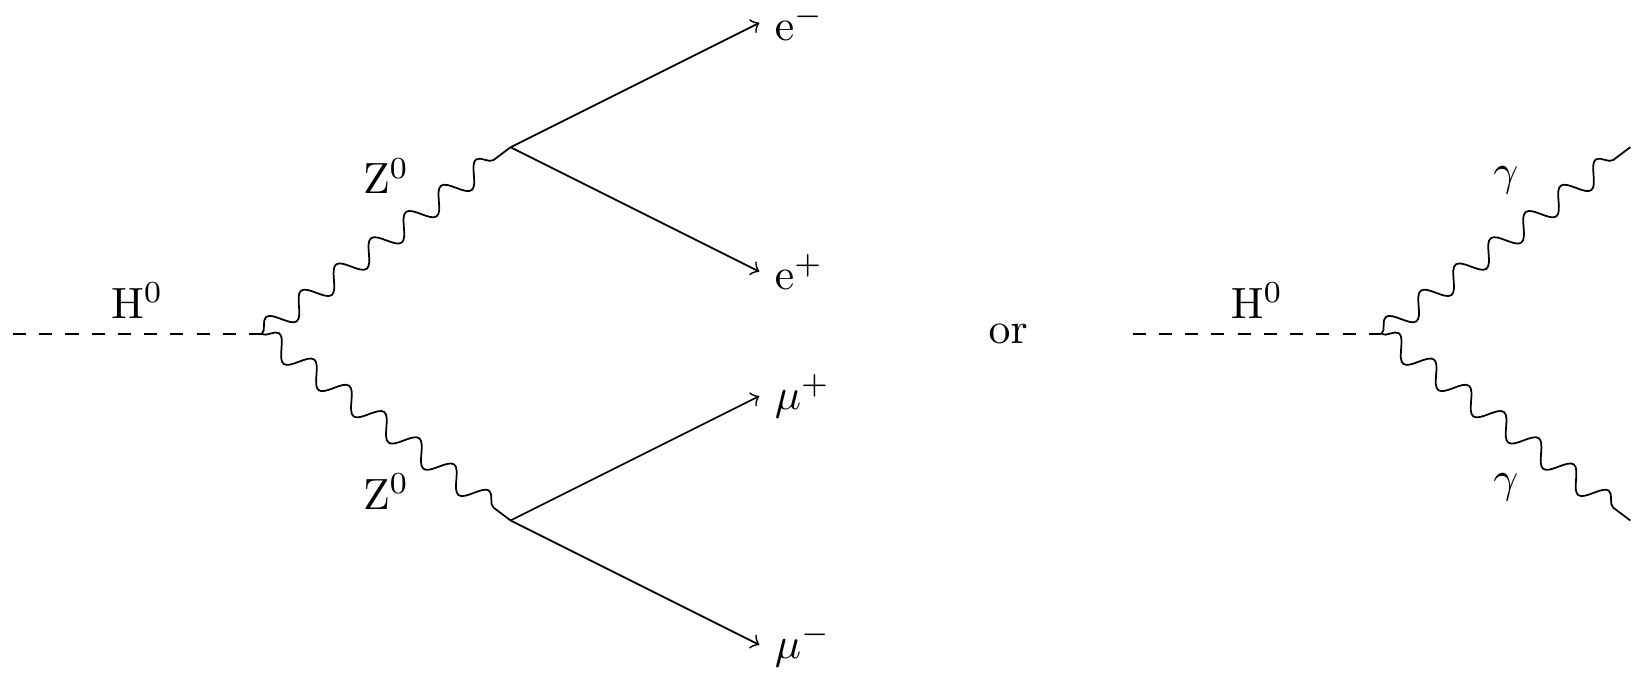
\includegraphics[scale=0.2]{HiggsDecay}
\end{center}

\subsection*{Feynman Diagrams}

\begin{center}
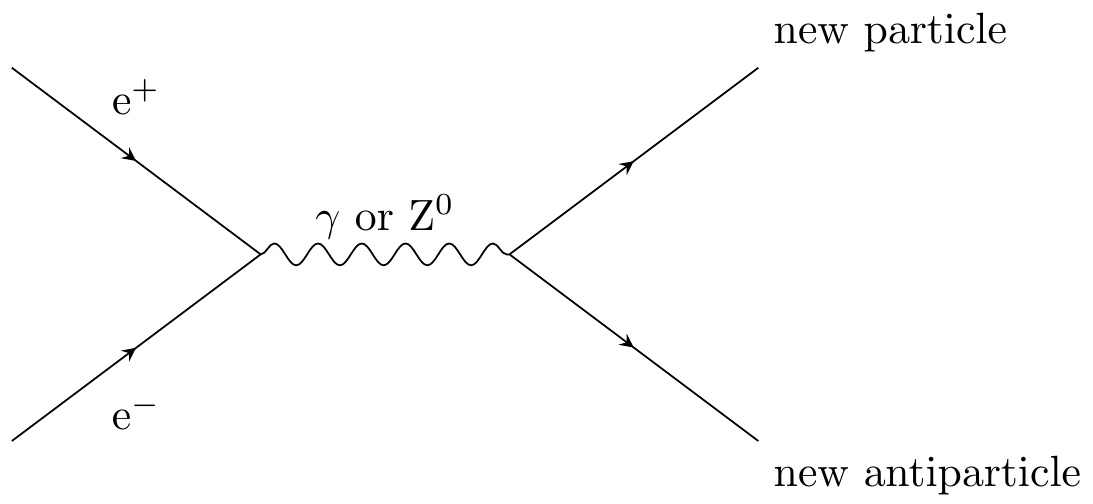
\includegraphics[scale=0.25]{Anihilation}
\end{center}

Electrons and positrons aren't quarks so this can't occur by the strong force. The total charge going in is 0 so the exchange particle must be neutral. This means that it is either a photon or a \zboson. Since it is a virtual particle it must eventually decay.

When drawing a Feynman diagram the typical axis are time increases upwards and space increases to the right. This means that if you rotate a diagram \SI{90}{\degree} clockwise and make all arrows going backwards into antiparticles then you get two equivalent diagrams

\begin{center}
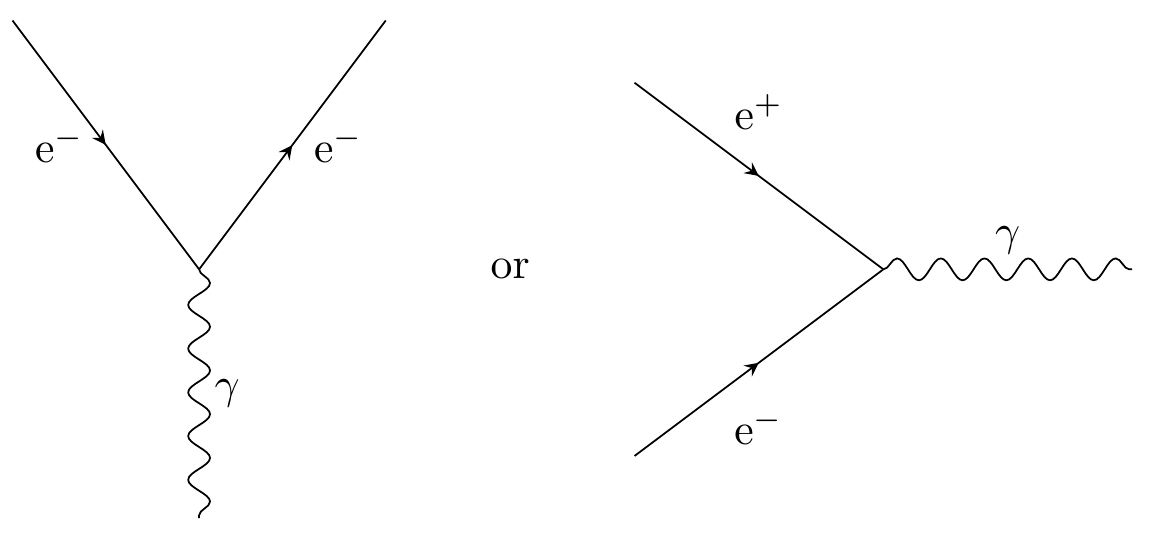
\includegraphics[scale=0.25]{AnihilationOrRedirect}
\end{center}

In Feynman diagrams it is standard to have antiparticles with their arrows going backwards in time.

\subsection*{Conservation Laws}

Some quantities are conserved in all (or at least most) reactions. This includes
\begin{itemize}
\item Charge (\(Q\) or \(C\))
\item Lepton number (\(L\)). Also each individual lepton generation number
\begin{itemize}
\item Electron number (\(L_\mathrm{e}\))
\item Muon number (\(L_\mu\))
\item Tauon number (\(L_\tau\))
\end{itemize}
\item Baryon number (\(B\))
\item Energy (\(E\))
\item Momentum (\(p\))
\end{itemize}

\begin{center}
\begin{tabular}{c|ccc}\hline
Number & +1 & 0 & -1\\\hline
\(L\) & \electron, \muonm, \tauonm & All other particles & \positron, \muonp, \tauonp\\
 & \neutrino[e], \neutrino[\mu], \neutrino[\tau] & & \antineutrino[e], \antineutrino[\mu], \antineutrino[\tau]\\\hline
\(L_e\) & \electron, \neutrino[e] & All other particles & \positron, \antineutrino[e]\\\hline
\(L_\mu\) & \muonm, \neutrino[\mu] & All other particles & \muonp, \antineutrino[\mu]\\\hline
\(L_\tau\) & \tauonm, \neutrino[\tau] & All other particles & \tauonp, \antineutrino[\tau]\\\hline
\(B\) & Baryons (3 quarks) & All other particles & Antibaryons (3 antiquarks)\\\hline
\end{tabular}
\end{center}
From this we give quarks a baryon number of \(+\frac 13\) and antiquarks a baryon number of \(-\frac 13\). This means that mesons (\quark\antiquark) have a baryon number of \(\frac 13-\frac 13=0\). Meson number is not a conserved number.

\section{}

Only the weak force can change quark flavour.

\begin{center}
\begin{tabular}{ccc}\hline
Force & Acts on & Relative Strength\\\hline
Strong force & Quarks and gluons & 1\\
EM & Charged particles & \num{e-2}\\
Weak & Fermions & \num{e-10	}\\
Gravity & Particles with mass & \num{e-40}\\\hline
\end{tabular}
\end{center}

Above a certain energy EM and weak forces are equally strong as there is so much energy that making a a photon or a \wpm/\zboson is just as easy so EM and weak forces merge into the electroweak (EW) force. We also think that the same happens with the strong force at even higher temperatures.

\begin{center}
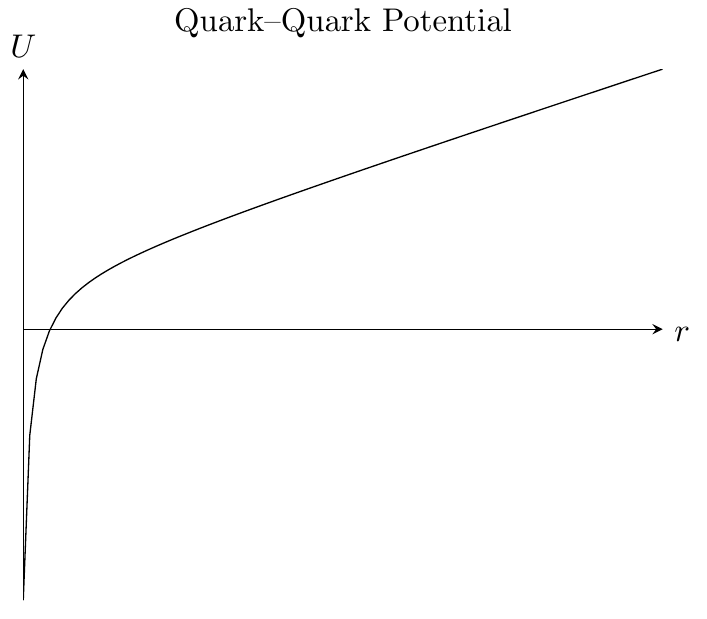
\includegraphics[scale=0.3]{QuarkQuarkPotential}
\end{center}

The quark--quark potential doesn't depend significantly on flavour, colour or whether it is a particle or antiparticle. Separating two quarks requires a lot of energy. This energy will form new particles which will then separate into multiple multi-quark systems rather than a single quark. This is called quark confinement.
\[\up\bar\up\ce{->}\up\quad\bar\up\ce{->}\up\bar\up\qquad\qquad\up\bar\up\]

\subsection*{Astrophysics}

\subsubsection*{Red/Blue Shift}

\[\frac{\lambda_{\mathrm{observed}}}{\lambda_{\mathrm{source}}}=\sqrt{\frac{1+v/c}{1-v/c}}\]
Where \(v\) is the relative speed between the observer and the source and \(v>0\) if they are moving appart. For \(v\ll c\) this reduces to
\[\frac{\Delta\lambda}{\lambda_{\mathrm{source}}}\approx\frac vc\]
Redshift \(z\) is a numerical value
\[z=\frac{\lambda_{\mathrm{obsv}}-\lambda_{\mathrm{source}}}{\lambda_{\mathrm{source}}}=\frac{f_{\mathrm{source}}-f_{\mathrm{obsv}}}{f_{\mathrm{obsv}}}\]
\[1+z=\frac{\lambda_{\mathrm{obsv}}}{\lambda_{\mathrm{source}}}=\frac{f_{\mathrm{source}}}{f_{\mathrm{obsv}}}\]

1 parsec (pc) \(\approx\) 3.3 light years (ly) \(\approx\num{3.086e16}\,\si{m}\)

Measurement of redshift of distant stars/galaxies shows that their velocity \(v\) is roughly proportional to the distance from us
\[v\propto r\implies v=H_0 r\]
where \(H_0\) is hubbles constant, \(H_0=\num{2.3e-18}\,\si{s^{-1}}\approx\SI{70}{kms^{-1}/Mpc}\). With all but a few local exceptions these galaxies are moving away from us.
\begin{example}
How far away is a galaxy with redshift \(z=0.1?\)

\[v=\num{3e7}\implies r=\frac{v}{H_0}=\num{1.3e25}\,\si{m}=\num{1.4e9}\,\si{ly}\]
\end{example}

Not only are all galaxies moving away from us but they are moving away from every thing else. The universe is growing isotropically (equally in all directions). This means the universe is expanding. This tracks back to the universe having 0 size at some point. Projecting backwards \(H_0^{-1}\approx14\) billion years which is a very basic approximation of the age of the universe. There is no center of the universe meaning the big bang happened everywhere simultaneously.

Gravity will slow expansion so the amount of gravity (and therefore matter) will affect the future of the universe. Is there enough matter to stop the universe from collapsing is an important question.

\section{}

A more sophisticated prediction for the future of the universe depends on how much gravity there is. This depends on how the universe compares to a critical density \(\rho_c\). A classical calculation gives
\[\rho_c=\frac{3H_0^2}{8\pi G}\]
The ratio of the actual density of the universe to this critical density is
\[\Omega=\frac{\rho}{\rho_c}\]
If the universe collapses it is called closed and \(\rho>\rho_c\implies\Omega>1\)

If the universe expands forever it is called open and \(\rho<\rho_c\implies\Omega<1\)

If the universe expands but stops after an infinite amount of time it is called flat and \(\rho=\rho_c\implies\Omega=1\)

\begin{center}
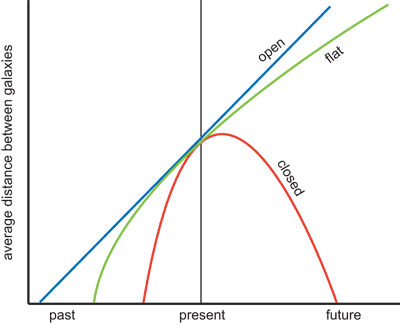
\includegraphics[scale=0.6]{FateOfTheUniverse}
\end{center}

If the universe is empty then the time from the start of the universe is \(H_0^{-1}\) seconds. If it is flat then it is \(\frac 23 H_0^{-1}\) seconds. One piece of evidence that the universe is flat is that the sum of all angles of a triangle in space time is \SI{180}{\degree}. A lot of evidence agrees that the universe is flat.

Our best guess for the age of the universe is \(13.799\pm0.021\) billion years old.

At the big bang the universe was very hot and very dense. At Planck scales quantum mechanics and general relativity break down. 

Before \num{e-11} \si{s} it is uncertain what happened. Before \num{e-37} \si{s} it is unknown what happened.

\(\sim\num{e-37}\) to \(\sim\num{e-32}\) the universe was in inflation. It expanded very rapidly by a factor of \num{e78}. This means that its speed is much greater than the speed of light. This is allowed as no matter went at this speed just the universe. This means that things became causally disconnected.

At \num{e-32} \si{s} inflation stops and the pressure/momentum causes expansion. The universe cools because it is expanding. At this point only quarks, gluons and photons can form.

At \num{e-12} \si{s} weak and EM split as the energy \(E\approx\num{e13}\approx m_{\wpm,\zboson}c^2\)

At \num{e-6} \si{s} it is cool enough to form neutrons and protons as the energy \(E\approx\SI{1}{GeV}\approx m_{p,n}c^2\) \((T\approx\num{e13}\,\si{K})\)

At 3 min it is cool enough to form elements (without electrons) as the energy \(E\approx\SI{1}{MeV}\approx BE(\ce{H})\) \((T\approx\num{e10}\,\si{K})\)

At 10 min it too cool to overcome the Coulomb barrier so new elements can't form. The universe is 75\% \ce{H}, 25\% \ce{He} and trace other elements.

At 380000 years it is cool enough that atoms (with electrons) because the energy \(E<IE\) \((T\approx\SI{3000}{K})\)

In the big bang hydrogen and helium were made. We can work out the total amount of baryonic matter \(\frac{\rho_{\mathrm{bar}}}{\rho_c}=\Omega_{\mathrm{bar}}=0.04\) since baryon number is conserved this is the same today.

After about 1 billion years hydrogen and helium come together under their own gravity. This contraction causes them to heat up.

One unit commonly used in astrophysics is a solar mass which is the mass of the sun and is equivalent to \num{2e30} \si{kg} and has the symbol \si{\solarmass}.

For sustained \ce{H} fusion we need \(M>\SI{0.08}{\solarmass}\). Once the star runs out of \ce{H} fusion stops so radiation pressure is lost so the star shrinks so it gets hotter. If \(M>\SI{0.5}{\solarmass}\) then \ce{He} fusion can occur and the star gets larger so the outer layers cool. This is a red giant. If it is heavy enough fusion of heavier elements occurs up to \ce{^56Fe}/\ce{^56Ni}. To get all the way to iron we need \(M>\SI{8}{\solarmass}\).

In supernovae and neutron star merges elements with atomic mass greater tha 56 can be formed.

\begin{center}
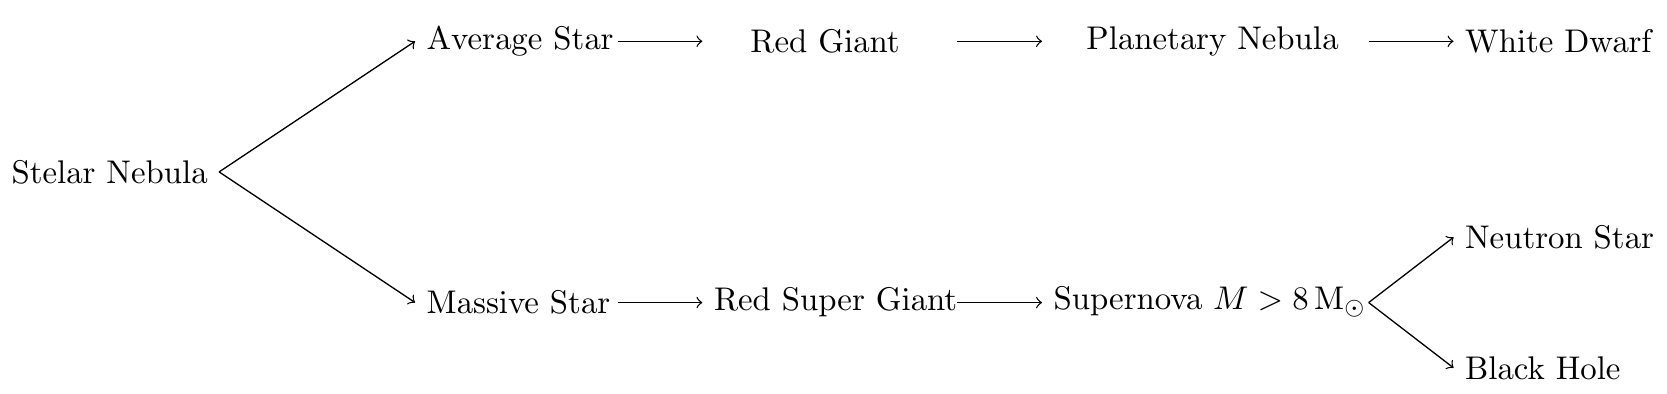
\includegraphics[scale=0.3]{LifeOfAStar}
\end{center}

\section{}

\begin{center}
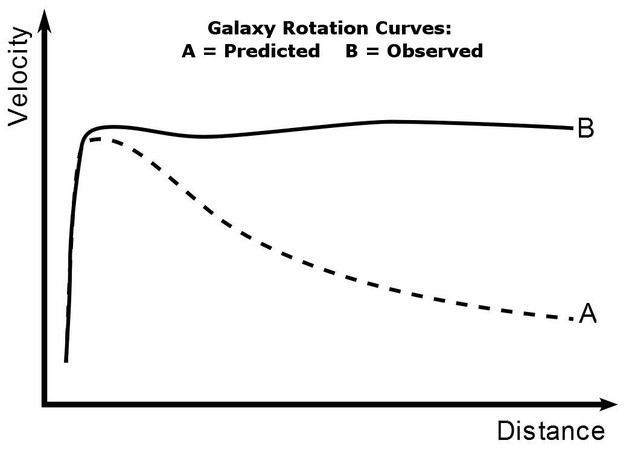
\includegraphics[scale=0.4]{GalaxyRotationSpeed}
\end{center}

For a spinning galaxy at a small distance \(r\) from the center we expect that the velocity \(v\propto r\). For a large distance we expect that equating centripetal and gravitational forces give the speed
\[\frac{mv^2}{r}=\frac{Gm_1m_2}{r^2}\implies v\propto\frac{1}{\sqrt{r}}\]
Our observation of the speed of the galaxy at these distances is higher than expected. This means that there must be more force than just the gravity of the rest of the galaxy which means that there must be more matter which we can't see so we call it dark matter. Dark matter is probably in a halo around the galaxy. The density ratio of visible matter is \(\Omega_\mathrm{lum}=0.03\). The density ratio of dark matter is \(\Omega_\mathrm{DM}=0.23\) which is about 8 times as much as visible matter.

No particle in the standard model fits the prediction of dark matter which is that it doesn't interact by the strong or EM force and hardly by the weak force if at all but is also very stable and much heavier than a neutrino. (It is possible that if we have measured the mass of a neutrino incorrectly or made an error in predicting the number of neutrinos that dark matter is neutrinos).

Super symmetry (SUSY) is a best guess at an extension for the standard model. It predicts every particle has a super symmetric counter part known as an sparticle (eg. a super symmetric quark is a squark, a supper symmetric lepton is a slepton) these have a different spin by \(\frac 12\) and solve some problems with the standard model.

To try to detect dark matter we put very sensitive detectors deep underground (to eliminate back ground radiation) we predict dark matter will interact a tiny bit by the weak force and if it does we should eventually detect it.

Some possible explanations for dark matter are
\begin{itemize}
\item WIMPS - weakly interacting massive particles
\item Pre-inflation black holes
\item Axions - particles needed to explain the lack of CP violation in most strong interactions
\item Modified gravity - general relativity doesn't work (unlikely)
\item Negative mass matter - mathematically allowed (probably, it could also be a bug in the code that did the computation)
\item Super symmetry
\end{itemize}

\subsection*{Binary Stellar Systems}

Binary stellar systems are what cause type 1a supernovae. A binary system is two stars orbiting each other. Typically they have masses in the range \(\SI{1}{\solarmass}<M<\SI{8}{\solarmass}\) and one of them is much heavier than the other so it evolves faster. After the hydrogen runs out the helium burns and it becomes a red giant. The smaller star becomes a white dwarf. Some layers from the red giant transfer to the white dwarf. When the mass of the white dwarf reaches \SI{1.44}{\solarmass} (Chandrasekhar limit) it implodes under its own weight as a type 1a supernova.

Since this occurs due to fundamental nuclear physics the explosions are almost identical for any 2 type 1a supernovae. This means that using their observed brightness we can tell how far away they are. We call a type 1a supernova a standard candle.

In 1998 scientists were studying distant (\(z=1\)) type 1a supernovae. The distance can be measured based on brightness and the speed can be calculated based on their redshift. The galaxies were receding more slowly faster than hubbles law predicts. This suggests distant things are accelerating away from us. To explain this we introduce dark energy. The density ratio of dark energy is \(\Omega_\lambda=0.73\). This means that the total ratio of densities is
\[\Omega_\mathrm{tot}=\Omega_\mathrm{bar}+\Omega_\mathrm{DM}+\Omega_\lambda=0.04+0.23+0.73=1.00\]
This means that the energy of the universe is 73\% dark energy, 23\% dark matter and 4\% normal matter which includes about 0.5\% stars and 0.3\% neutrinos. The fact that dark energy causes acceleration means that even if \(\Omega_\mathrm{tot}=1\) the universe will still be open and expand forever.

It is possible that dark matter and dark energy are the same. Dark matter explains galactic scale motion and dark energy explains universe scale motion. Dark energy is a lot like inflation.

There are several goal in physics of finding a combined theory of the different forces.
\begin{itemize}
\item EM + weak force = Electro weak theory (EW)
\item EW + strong force = Grand unified theory (GUT)
\item GUT + gravity = Theory of everything (TOE)
\end{itemize}
\end{document}